\documentclass[11pt, letterpaper]{article}

% Fonts and Encoding
\usepackage[utf8]{inputenc}
\usepackage[T1]{fontenc}
\usepackage{lmodern} % High-quality Latin Modern vector font

% Math and Symbols
\usepackage{amsmath, amssymb, amsthm, amsfonts, mathrsfs, mathtools}

% Layout and Geometry
\usepackage{geometry}
\geometry{letterpaper, margin=1in}
\setlength{\parindent}{0pt}
\setlength{\parskip}{0.6em}

% Formatting and Graphics
\usepackage{graphicx, xcolor, enumitem, booktabs, array, tabularx}

% TikZ for Illustrations
\usepackage{tikz}
\usetikzlibrary{arrows.meta, positioning, shapes.geometric, calc, backgrounds, matrix}

% Clickable Links and TOC
\usepackage{hyperref}
\hypersetup{
    colorlinks=true,
    linkcolor=blue,
    filecolor=magenta,      
    urlcolor=cyan,
    pdftitle={Advanced Mathematics Topic},
}

% Theorem Environments
\newtheorem{theorem}{Theorem}[section]
\newtheorem{lemma}[theorem]{Lemma}
\newtheorem{proposition}[theorem]{Proposition}
\newtheorem{corollary}[theorem]{Corollary}
\theoremstyle{definition}
\newtheorem{definition}{Definition}[section]
\newtheorem{axiom}{Axiom}[section]
\newtheorem{example}{Example}[section]
\theoremstyle{remark}
\newtheorem{remark}{Remark}[section]

% Custom Commands (Enforced standard notation)
\newcommand{\R}{\mathbb{R}}
\newcommand{\N}{\mathbb{N}}
\newcommand{\Z}{\mathbb{Z}}
\newcommand{\Q}{\mathbb{Q}}
\newcommand{\E}{\mathbb{E}}
\newcommand{\Prob}{\mathbb{P}}
\newcommand{\F}{\mathcal{F}}

\title{Mastering Orthogonal Sets and Projections: Practice Problem Sets and Detailed Solutions}
\author{Tashfeen Omran}
\date{November 16, 2026}

\begin{document}

\maketitle
\tableofcontents
\newpage

\section{Concept Checklist and Question Mapping}

The table below catalogs every core concept, theorem, algebraic manipulation, real-world application, and diagnostic pitfall from \textit{Mastering Orthogonal Sets and Projections}, mapped directly to the $36$ practice problems in this document. Heavier weight is assigned to conceptually demanding topics such as projections, matrix proofs, Gram-Schmidt orthogonalization, least-squares modeling, and error diagnostics.

\renewcommand{\arraystretch}{1.5}
\begin{tabularx}{\textwidth}{>{\raggedright\arraybackslash}p{4.3cm} >{\raggedright\arraybackslash}X >{\raggedright\arraybackslash}p{2.6cm}}
\toprule
\textbf{Concept / Problem Type} & \textbf{Core Formulas, Techniques, and Pitfalls} & \textbf{Relevant Problems} \\
\midrule
Determining Orthogonal Sets \& Parameters & Check all pairwise dot products $\mathbf{v}_i \cdot \mathbf{v}_j = 0$ ($i \neq j$); solve parameter constraints and verify every pair. & 1, 2, 3, 4 \\
\addlinespace[4pt]
The Zero Vector Trap \& Linear Independence & Since $\mathbf{0} \cdot \mathbf{v} = 0$ for all $\mathbf{v}$, a set containing $\mathbf{0}$ can be orthogonal, but is never linearly independent or orthonormal. & 3, 19, 23 \\
\addlinespace[4pt]
Orthogonal Bases \& Decoupled Weights (Theorems 4 \& 5) & Nonzero orthogonal vectors are linearly independent; basis weights decouple cleanly as $c_i = \frac{\mathbf{x} \cdot \mathbf{u}_i}{\mathbf{u}_i \cdot \mathbf{u}_i}$ without row reduction. & 5, 6, 7, 8, 20, 23, 35 \\
\addlinespace[4pt]
Orthogonal Projections onto Lines \& Subspaces & Compute $\hat{\mathbf{y}} = \operatorname{proj}_L \mathbf{y} = \frac{\mathbf{y} \cdot \mathbf{u}}{\mathbf{u} \cdot \mathbf{u}}\mathbf{u}$; scaling invariance $\operatorname{proj}_{c\mathbf{u}}\mathbf{y} = \operatorname{proj}_{\mathbf{u}}\mathbf{y}$ ($c \neq 0$); multi-vector orthogonal projection. & 9, 10, 12, 22, 26, 34 \\
\addlinespace[4pt]
Orthogonal Decomposition \& Error Check & Decompose $\mathbf{y} = \hat{\mathbf{y}} + \mathbf{z}$ with $\hat{\mathbf{y}} \in W$ and $\mathbf{z} = \mathbf{y} - \hat{\mathbf{y}} \in W^\perp$; always verify $\mathbf{z} \cdot \mathbf{u}_i = 0$. & 11, 12, 27 \\
\addlinespace[4pt]
Distance to a Subspace \& Pythagorean Theorem & Distance is $d = \|\mathbf{y} - \hat{\mathbf{y}}\| = \|\mathbf{z}\|$ (never $\|\hat{\mathbf{y}}\|$); satisfies $\|\mathbf{y}\|^2 = \|\hat{\mathbf{y}}\|^2 + \|\mathbf{z}\|^2$. & 13, 14, 22, 34 \\
\addlinespace[4pt]
Reflection Operators \& Linear Transformations & $\operatorname{refl}_L \mathbf{y} = 2\operatorname{proj}_L \mathbf{y} - \mathbf{y}$; prove linearity of $\operatorname{proj}_L$ and $\operatorname{refl}_L$, compute standard matrices, and verify $\|\operatorname{refl}_L \mathbf{y}\| = \|\mathbf{y}\|$. & 15, 26 \\
\addlinespace[4pt]
Orthonormal Sets \& Normalization & Requires orthogonality \textit{and} unit length ($\|\mathbf{u}_i\| = 1$); normalize via $\mathbf{u}_i = \mathbf{v}_i / \|\mathbf{v}_i\|$, which preserves orthogonality. & 16, 17, 18, 20, 36 \\
\addlinespace[4pt]
Norm \& Inner Product Preservation (Theorem 7) & If $U$ has orthonormal columns ($U^T U = I_n$), then $(U\mathbf{x}) \cdot (U\mathbf{y}) = \mathbf{x} \cdot \mathbf{y}$ and $\|U\mathbf{x}\| = \|\mathbf{x}\|$. & 24, 28 \\
\addlinespace[4pt]
Square Orthogonal Matrices ($U^{-1} = U^T$) & Must be square ($n \times n$); $U^T U = U U^T = I_n$; invertible with $U^{-1} = U^T$; orthonormal rows; closed under multiplication ($UV$). & 21, 25, 26, 36 \\
\addlinespace[4pt]
Rectangular Matrices ($U^T U$ vs.\ $U U^T$) & For $m \times n$ ($m > n$), $U^T U = I_n$ while $U U^T \neq I_m$ projects onto $\operatorname{Col}(A)$; $(A^T A)_{ij} = \mathbf{a}_i \cdot \mathbf{a}_j$ determines orthogonality. & 21, 27, 28, 31 \\
\addlinespace[4pt]
The Gram-Schmidt Process & Convert a non-orthogonal basis to an orthogonal basis via $\mathbf{v}_k = \mathbf{x}_k - \sum_{i=1}^{k-1} \frac{\mathbf{x}_k \cdot \mathbf{v}_i}{\mathbf{v}_i \cdot \mathbf{v}_i}\mathbf{v}_i$, then normalize if needed. & 29, 30 \\
\addlinespace[4pt]
General Projection Matrices & Compute $P = A(A^T A)^{-1}A^T$, verify $P^2 = P$ and $P^T = P$, and show $P$ collapses to $U U^T$ for orthonormal columns. & 27, 31 \\
\addlinespace[4pt]
Ordinary Least Squares (OLS) \& Normal Equations & Minimize $\|\mathbf{y} - X\boldsymbol{\beta}\|^2$ via $X^T \boldsymbol{\epsilon} = \mathbf{0} \implies X^T X \hat{\boldsymbol{\beta}} = X^T \mathbf{y}$; simplifies to $\hat{\boldsymbol{\beta}} = Q^T \mathbf{y}$ when $Q$ has orthonormal columns. & 32 \\
\addlinespace[4pt]
Integral Inner Products \& Fourier Decoupling & Verify orthogonality of $\{1, \cos(x), \sin(x)\}$ under $\langle f, g \rangle = \int_{-\pi}^{\pi} f(x)g(x)\,dx$ and project functions using Theorem 5 weights. & 33 \\
\addlinespace[4pt]
Diagnostic Testing (``Find the Flaw'') & Identify wrong projection denominators ($\mathbf{y}\cdot\mathbf{y}$), wrong distance norms ($\|\hat{\mathbf{y}}\|$), Theorem 5 on non-orthogonal bases, and $U^T U = I$ traps. & 34, 35, 36 \\
\bottomrule
\end{tabularx}

\newpage

\section{Problem Sets}

\subsection{Determining Orthogonal Sets and Parameter Constraints}

\textbf{Problem 1.} Determine whether the set $\{\mathbf{v}_1, \mathbf{v}_2, \mathbf{v}_3\}$ in $\mathbb{R}^3$ is orthogonal, where
\[
\mathbf{v}_1 = \begin{bmatrix} 2 \\ -1 \\ 3 \end{bmatrix}, \qquad
\mathbf{v}_2 = \begin{bmatrix} 1 \\ 5 \\ 1 \end{bmatrix}, \qquad
\mathbf{v}_3 = \begin{bmatrix} -4 \\ 1 \\ 3 \end{bmatrix}.
\]

\textbf{Problem 2.} Determine whether the set $\{\mathbf{v}_1, \mathbf{v}_2, \mathbf{v}_3\}$ in $\mathbb{R}^4$ is orthogonal, where
\[
\mathbf{v}_1 = \begin{bmatrix} 1 \\ -2 \\ 3 \\ -1 \end{bmatrix}, \qquad
\mathbf{v}_2 = \begin{bmatrix} 3 \\ 2 \\ 1 \\ 2 \end{bmatrix}, \qquad
\mathbf{v}_3 = \begin{bmatrix} 1 \\ 6 \\ 1 \\ -8 \end{bmatrix}.
\]

\textbf{Problem 3.} Consider the set $S = \{\mathbf{v}_1, \mathbf{v}_2, \mathbf{v}_3\}$ in $\mathbb{R}^4$, where
\[
\mathbf{v}_1 = \begin{bmatrix} 4 \\ -1 \\ 2 \\ 3 \end{bmatrix}, \qquad
\mathbf{v}_2 = \begin{bmatrix} 0 \\ 0 \\ 0 \\ 0 \end{bmatrix}, \qquad
\mathbf{v}_3 = \begin{bmatrix} 1 \\ 3 \\ -2 \\ 1 \end{bmatrix}.
\]
(a) Is $S$ an orthogonal set? \\
(b) Is $S$ linearly independent? Can $S$ be normalized to form an orthonormal set? Explain clearly.

\textbf{Problem 4.} Find all values of the real parameters $a$ and $b$ such that the set $\{\mathbf{v}_1, \mathbf{v}_2, \mathbf{v}_3\}$ is orthogonal, where
\[
\mathbf{v}_1 = \begin{bmatrix} 1 \\ 2 \\ -1 \end{bmatrix}, \qquad
\mathbf{v}_2 = \begin{bmatrix} a \\ 1 \\ 4 \end{bmatrix}, \qquad
\mathbf{v}_3 = \begin{bmatrix} 3 \\ b \\ -1 \end{bmatrix}.
\]

\subsection{Orthogonal Bases and Linear Combinations}

\textbf{Problem 5.} Show that $\{\mathbf{u}_1, \mathbf{u}_2\}$ is an orthogonal basis for $\mathbb{R}^2$, and express $\mathbf{x}$ as a linear combination of $\mathbf{u}_1$ and $\mathbf{u}_2$, where
\[
\mathbf{u}_1 = \begin{bmatrix} 4 \\ -2 \end{bmatrix}, \qquad
\mathbf{u}_2 = \begin{bmatrix} 3 \\ 6 \end{bmatrix}, \qquad
\mathbf{x} = \begin{bmatrix} 7 \\ -6 \end{bmatrix}.
\]

\textbf{Problem 6.} Show that $\{\mathbf{u}_1, \mathbf{u}_2, \mathbf{u}_3\}$ is an orthogonal basis for $\mathbb{R}^3$, and express $\mathbf{x}$ as a linear combination of $\mathbf{u}_1, \mathbf{u}_2, \mathbf{u}_3$, where
\[
\mathbf{u}_1 = \begin{bmatrix} 1 \\ 1 \\ 1 \end{bmatrix}, \qquad
\mathbf{u}_2 = \begin{bmatrix} 1 \\ -1 \\ 0 \end{bmatrix}, \qquad
\mathbf{u}_3 = \begin{bmatrix} 1 \\ 1 \\ -2 \end{bmatrix}, \qquad
\mathbf{x} = \begin{bmatrix} 4 \\ -3 \\ 5 \end{bmatrix}.
\]

\textbf{Problem 7.} Show that $\{\mathbf{u}_1, \mathbf{u}_2, \mathbf{u}_3, \mathbf{u}_4\}$ is an orthogonal basis for $\mathbb{R}^4$, and express $\mathbf{x}$ as a linear combination of the basis vectors, where
\[
\mathbf{u}_1 = \begin{bmatrix} 1 \\ 1 \\ 1 \\ 1 \end{bmatrix}, \qquad
\mathbf{u}_2 = \begin{bmatrix} 1 \\ 1 \\ -1 \\ -1 \end{bmatrix}, \qquad
\mathbf{u}_3 = \begin{bmatrix} 1 \\ -1 \\ 0 \\ 0 \end{bmatrix}, \qquad
\mathbf{u}_4 = \begin{bmatrix} 0 \\ 0 \\ 1 \\ -1 \end{bmatrix}, \qquad
\mathbf{x} = \begin{bmatrix} 3 \\ -1 \\ 6 \\ 2 \end{bmatrix}.
\]

\textbf{Problem 8.} Let $\mathbf{u}_1 = \begin{bmatrix} 1 \\ -2 \\ 2 \end{bmatrix}$ and $\mathbf{u}_2 = \begin{bmatrix} 2 \\ 1 \\ 0 \end{bmatrix}$. \\
(a) Verify that $\mathbf{u}_1 \cdot \mathbf{u}_2 = 0$, and find the unique vector $\mathbf{u}_3 \in \mathbb{R}^3$ with first component equal to $2$ such that $\{\mathbf{u}_1, \mathbf{u}_2, \mathbf{u}_3\}$ is an orthogonal basis for $\mathbb{R}^3$. \\
(b) Express $\mathbf{x} = \begin{bmatrix} 1 \\ 3 \\ -4 \end{bmatrix}$ as a linear combination of $\mathbf{u}_1, \mathbf{u}_2, \mathbf{u}_3$.

\subsection{Orthogonal Projections, Decompositions, Reflections, and Distances}

\textbf{Problem 9.} Compute the orthogonal projection $\hat{\mathbf{y}}$ of $\mathbf{y} = \begin{bmatrix} 5 \\ -3 \end{bmatrix}$ onto the line $L$ through $\mathbf{u} = \begin{bmatrix} 2 \\ 4 \end{bmatrix}$ and the origin.

\textbf{Problem 10.} Compute the orthogonal projection $\hat{\mathbf{y}}$ of $\mathbf{y} = \begin{bmatrix} 5 \\ -1 \\ 7 \end{bmatrix}$ onto the line $L$ through $\mathbf{u} = \begin{bmatrix} 1 \\ -2 \\ 3 \end{bmatrix}$ and the origin, and verify that $\mathbf{y} - \hat{\mathbf{y}}$ is orthogonal to $\mathbf{u}$.

\textbf{Problem 11.} Let $\mathbf{y} = \begin{bmatrix} 1 \\ 4 \end{bmatrix}$ and $\mathbf{u} = \begin{bmatrix} 3 \\ 1 \end{bmatrix}$. Write $\mathbf{y}$ as the sum of two orthogonal vectors $\hat{\mathbf{y}} + \mathbf{z}$, where $\hat{\mathbf{y}} \in \operatorname{Span}\{\mathbf{u}\}$ and $\mathbf{z}$ is orthogonal to $\mathbf{u}$.

\textbf{Problem 12.} Let $W = \operatorname{Span}\{\mathbf{u}_1, \mathbf{u}_2\} \subset \mathbb{R}^3$, where $\mathbf{u}_1 = \begin{bmatrix} 1 \\ 2 \\ 0 \end{bmatrix}$ and $\mathbf{u}_2 = \begin{bmatrix} -2 \\ 1 \\ 5 \end{bmatrix}$, and let $\mathbf{y} = \begin{bmatrix} 3 \\ 1 \\ -2 \end{bmatrix}$. \\
(a) Verify that $\{\mathbf{u}_1, \mathbf{u}_2\}$ is an orthogonal basis for $W$. \\
(b) Compute $\hat{\mathbf{y}} = \operatorname{proj}_W \mathbf{y} = \frac{\mathbf{y} \cdot \mathbf{u}_1}{\mathbf{u}_1 \cdot \mathbf{u}_1}\mathbf{u}_1 + \frac{\mathbf{y} \cdot \mathbf{u}_2}{\mathbf{u}_2 \cdot \mathbf{u}_2}\mathbf{u}_2$. \\
(c) Write $\mathbf{y} = \hat{\mathbf{y}} + \mathbf{z}$, and verify explicitly that $\mathbf{z}$ is orthogonal to both $\mathbf{u}_1$ and $\mathbf{u}_2$ (hence $\mathbf{z} \in W^\perp$).

\textbf{Problem 13.} Compute the distance from $\mathbf{y} = \begin{bmatrix} -2 \\ 9 \end{bmatrix}$ to the line $L$ through $\mathbf{u} = \begin{bmatrix} 3 \\ 4 \end{bmatrix}$ and the origin.

\textbf{Problem 14.} Compute the distance $d$ from $\mathbf{y} = \begin{bmatrix} 3 \\ -1 \\ 5 \end{bmatrix}$ to the line $L$ through $\mathbf{u} = \begin{bmatrix} 2 \\ 1 \\ 2 \end{bmatrix}$ and the origin. Verify that the Pythagorean identity $\|\mathbf{y}\|^2 = \|\hat{\mathbf{y}}\|^2 + d^2$ holds.

\textbf{Problem 15.} Let $L = \operatorname{Span}\{\mathbf{u}\}$ in $\mathbb{R}^2$, where $\mathbf{u} = \begin{bmatrix} 2 \\ 1 \end{bmatrix}$, and let $\mathbf{y} = \begin{bmatrix} 1 \\ 3 \end{bmatrix}$. \\
(a) Compute the orthogonal reflection $\operatorname{refl}_L \mathbf{y} = 2\operatorname{proj}_L \mathbf{y} - \mathbf{y}$. \\
(b) Verify that $\|\operatorname{refl}_L \mathbf{y}\| = \|\mathbf{y}\|$ and that $\operatorname{refl}_L \mathbf{y} - \hat{\mathbf{y}} = -(\mathbf{y} - \hat{\mathbf{y}})$.

\subsection{Orthonormal Sets and Normalization}

\textbf{Problem 16.} Determine whether the set $\{\mathbf{v}_1, \mathbf{v}_2\}$ in $\mathbb{R}^3$ is orthonormal. If it is only orthogonal, normalize the vectors to form an orthonormal set:
\[
\mathbf{v}_1 = \begin{bmatrix} 1/2 \\ -1/2 \\ 1/2 \end{bmatrix}, \qquad
\mathbf{v}_2 = \begin{bmatrix} 1/3 \\ 1/3 \\ 0 \end{bmatrix}.
\]

\textbf{Problem 17.} Determine whether the set $\{\mathbf{v}_1, \mathbf{v}_2, \mathbf{v}_3\}$ in $\mathbb{R}^3$ is orthonormal:
\[
\mathbf{v}_1 = \begin{bmatrix} 2/\sqrt{14} \\ 1/\sqrt{14} \\ -3/\sqrt{14} \end{bmatrix}, \qquad
\mathbf{v}_2 = \begin{bmatrix} 1/\sqrt{5} \\ -2/\sqrt{5} \\ 0 \end{bmatrix}, \qquad
\mathbf{v}_3 = \begin{bmatrix} 6/\sqrt{70} \\ 3/\sqrt{70} \\ 5/\sqrt{70} \end{bmatrix}.
\]

\textbf{Problem 18.} Let $\mathbf{v}_1 = \begin{bmatrix} 1 \\ 2 \\ 2 \end{bmatrix}$ and $\mathbf{v}_2 = \begin{bmatrix} 2 \\ -1 \\ 0 \end{bmatrix}$. \\
(a) Verify that $\mathbf{v}_1$ and $\mathbf{v}_2$ are orthogonal, and normalize them to obtain unit vectors $\mathbf{u}_1$ and $\mathbf{u}_2$. \\
(b) Find a third unit vector $\mathbf{u}_3 \in \mathbb{R}^3$ with positive first entry such that $\{\mathbf{u}_1, \mathbf{u}_2, \mathbf{u}_3\}$ forms an orthonormal basis for $\mathbb{R}^3$.

\subsection{Conceptual Analysis: True or False}

\textbf{Problem 19.} Determine whether each statement is True or False, and justify your answer with a proof or counterexample: \\
(a) Every linearly independent set of vectors in $\mathbb{R}^n$ is orthogonal. \\
(b) Every orthogonal set of vectors in $\mathbb{R}^n$ is linearly independent.

\textbf{Problem 20.} Determine whether each statement is True or False, and justify your answer: \\
(a) If $\{\mathbf{v}_1, \mathbf{v}_2\}$ is an orthogonal set of nonzero vectors, then normalizing each vector preserves orthogonality and yields an orthonormal set. \\
(b) If $\{\mathbf{u}_1, \dots, \mathbf{u}_p\}$ is an orthogonal basis for a subspace $W \subseteq \mathbb{R}^n$ and $\mathbf{x} \in W$, then $\mathbf{x} = c_1\mathbf{u}_1 + \dots + c_p\mathbf{u}_p$ where $c_j = \frac{\mathbf{x} \cdot \mathbf{u}_j}{\mathbf{u}_j \cdot \mathbf{u}_j}$.

\textbf{Problem 21.} Determine whether each statement is True or False, and justify your answer: \\
(a) If $U$ is a $4 \times 3$ matrix with orthonormal columns, then $U$ is an orthogonal matrix and satisfies $U U^T = I_4$. \\
(b) If $U$ is an $n \times n$ matrix with orthonormal columns, then $U$ is invertible and $U^{-1} = U^T$.

\textbf{Problem 22.} Determine whether each statement is True or False, and justify your answer: \\
(a) For any nonzero vector $\mathbf{v} \in \mathbb{R}^n$, any nonzero scalar $c \in \mathbb{R}$, and any $\mathbf{y} \in \mathbb{R}^n$, we have $\operatorname{proj}_{c\mathbf{v}} \mathbf{y} = \operatorname{proj}_{\mathbf{v}} \mathbf{y}$. \\
(b) For any vector $\mathbf{y} \in \mathbb{R}^n$ and any line $L = \operatorname{Span}\{\mathbf{u}\}$ with $\mathbf{u} \neq \mathbf{0}$, the distance from $\mathbf{y}$ to $L$ is $\|\operatorname{proj}_L \mathbf{y}\|$.

\subsection{Proofs, Linear Transformations, and Matrix Properties}

\textbf{Problem 23.} (a) Prove Theorem 4: If $S = \{\mathbf{v}_1, \mathbf{v}_2, \dots, \mathbf{v}_p\}$ is an orthogonal set of nonzero vectors in $\mathbb{R}^n$, then $S$ is linearly independent. \\
(b) Explain why any subspace $W \subseteq \mathbb{R}^n$ spanned by $n$ nonzero orthogonal vectors must satisfy $W = \mathbb{R}^n$.

\textbf{Problem 24.} Let $U$ be an $m \times n$ matrix with orthonormal columns. Using the matrix-transpose identity $\mathbf{u} \cdot \mathbf{v} = \mathbf{u}^T \mathbf{v}$, prove Theorem 7: for all $\mathbf{x}, \mathbf{y} \in \mathbb{R}^n$, \\
(a) $(U\mathbf{x}) \cdot (U\mathbf{y}) = \mathbf{x} \cdot \mathbf{y}$ (and deduce that $U\mathbf{x} \perp U\mathbf{y}$ whenever $\mathbf{x} \perp \mathbf{y}$); \\
(b) $\|U\mathbf{x}\| = \|\mathbf{x}\|$.

\textbf{Problem 25.} Let $U$ and $V$ be $n \times n$ orthogonal matrices (square matrices with orthonormal columns). \\
(a) Explain why $U$ is invertible and $U^{-1} = U^T$. \\
(b) Prove that the rows of $U$ form an orthonormal basis of $\mathbb{R}^n$. \\
(c) Prove that the matrix product $UV$ is also an orthogonal matrix.

\textbf{Problem 26.} Let $\mathbf{u} \in \mathbb{R}^n$ be a nonzero vector and $L = \operatorname{Span}\{\mathbf{u}\}$. \\
(a) Prove that both $T(\mathbf{x}) = \operatorname{proj}_L \mathbf{x} = \frac{\mathbf{x} \cdot \mathbf{u}}{\mathbf{u} \cdot \mathbf{u}}\mathbf{u}$ and $R(\mathbf{x}) = 2\operatorname{proj}_L \mathbf{x} - \mathbf{x}$ are linear transformations from $\mathbb{R}^n$ to $\mathbb{R}^n$. \\
(b) Let $n = 2$ and $\mathbf{u} = \begin{bmatrix} 3 \\ 4 \end{bmatrix}$. Find the $2 \times 2$ standard matrices $[T]$ and $[R]$ such that $T(\mathbf{x}) = [T]\mathbf{x}$ and $R(\mathbf{x}) = [R]\mathbf{x}$, and verify directly that $[R]$ is an orthogonal matrix.

\textbf{Problem 27.} Let $A = \begin{bmatrix} 1 & -2 \\ 2 & -1 \\ 2 & 2 \end{bmatrix}$. Observe that the columns of $A$ are orthogonal, and let $U$ be the $3 \times 2$ matrix obtained by normalizing each column of $A$. \\
(a) Compute $U$, $U^T U$, and $U U^T$. Explain why $U^T U = I_2$ while $U U^T \neq I_3$. \\
(b) For an arbitrary vector $\mathbf{y} \in \mathbb{R}^3$, let $\mathbf{p} = U U^T \mathbf{y}$ and $\mathbf{z} = \mathbf{y} - \mathbf{p}$. Prove in general that $\mathbf{p} \in \operatorname{Col}(A)$ and $\mathbf{z} \in (\operatorname{Col}(A))^\perp$. \\
(c) Compute $\mathbf{p}$ and $\mathbf{z}$ explicitly for $\mathbf{y} = \begin{bmatrix} 3 \\ 3 \\ 9 \end{bmatrix}$ and verify that $\mathbf{z}$ is orthogonal to both columns of $A$.

\textbf{Problem 28.} Let $A$ be any $m \times n$ matrix with columns $\mathbf{a}_1, \mathbf{a}_2, \dots, \mathbf{a}_n \in \mathbb{R}^m$. \\
(a) Prove that the $(i, j)$-entry of $A^T A$ equals $\mathbf{a}_i \cdot \mathbf{a}_j$. \\
(b) Deduce that the columns of $A$ form an orthogonal set if and only if $A^T A$ is a diagonal matrix. \\
(c) Deduce that the columns of $A$ form an orthonormal set if and only if $A^T A = I_n$.

\subsection{Advanced Applications: Gram-Schmidt, Projection Matrices, Least Squares, and Function Spaces}

\textbf{Problem 29.} Let $W = \operatorname{Span}\{\mathbf{x}_1, \mathbf{x}_2\} \subset \mathbb{R}^3$, where $\mathbf{x}_1 = \begin{bmatrix} 1 \\ 2 \\ 2 \end{bmatrix}$ and $\mathbf{x}_2 = \begin{bmatrix} 3 \\ 0 \\ 3 \end{bmatrix}$. Use the Gram-Schmidt process to find: \\
(a) an orthogonal basis $\{\mathbf{v}_1, \mathbf{v}_2\}$ for $W$; \\
(b) an orthonormal basis $\{\mathbf{u}_1, \mathbf{u}_2\}$ for $W$.

\textbf{Problem 30.} Apply the Gram-Schmidt process to the linearly independent set $\{\mathbf{x}_1, \mathbf{x}_2, \mathbf{x}_3\}$ in $\mathbb{R}^3$ to construct an orthogonal basis $\{\mathbf{v}_1, \mathbf{v}_2, \mathbf{v}_3\}$ for $\mathbb{R}^3$, where
\[
\mathbf{x}_1 = \begin{bmatrix} 1 \\ 1 \\ 0 \end{bmatrix}, \qquad
\mathbf{x}_2 = \begin{bmatrix} 2 \\ 0 \\ 1 \end{bmatrix}, \qquad
\mathbf{x}_3 = \begin{bmatrix} 1 \\ 3 \\ 5 \end{bmatrix}.
\]
Verify directly that all pairwise dot products among $\mathbf{v}_1, \mathbf{v}_2, \mathbf{v}_3$ equal zero.

\textbf{Problem 31.} Let $A = \begin{bmatrix} 1 & 0 \\ 1 & 1 \\ 0 & 1 \end{bmatrix}$, whose columns are linearly independent but not orthogonal. \\
(a) Compute the standard projection matrix $P = A(A^T A)^{-1}A^T$ onto $\operatorname{Col}(A)$. \\
(b) Verify directly that $P^2 = P$ and $P^T = P$, and use $P$ to compute the projection $\hat{\mathbf{y}} = P\mathbf{y}$ of $\mathbf{y} = \begin{bmatrix} 3 \\ 0 \\ 3 \end{bmatrix}$ onto $\operatorname{Col}(A)$. \\
(c) Prove algebraically that if $U$ is any $m \times n$ matrix with orthonormal columns, then $P_U = U U^T$ satisfies $P_U^2 = P_U$ and $P_U^T = P_U$, and explain why $A(A^T A)^{-1} A^T$ collapses to $U U^T$ when $A = U$.

\textbf{Problem 32.} In an Ordinary Least Squares (OLS) regression problem with $N = 4$ observations and $p = 2$ features, the design matrix $X \in \mathbb{R}^{4 \times 2}$ and target vector $\mathbf{y} \in \mathbb{R}^4$ are
\[
X = \begin{bmatrix} 1 & 0 \\ 1 & 1 \\ 1 & 2 \\ 1 & 3 \end{bmatrix}, \qquad
\mathbf{y} = \begin{bmatrix} 2 \\ 2 \\ 4 \\ 8 \end{bmatrix}.
\]
We seek a parameter vector $\hat{\boldsymbol{\beta}} \in \mathbb{R}^2$ minimizing the squared error loss $\mathcal{L}(\boldsymbol{\beta}) = \|\mathbf{y} - X\boldsymbol{\beta}\|^2$. \\
(a) Using the geometric condition that the residual $\boldsymbol{\epsilon} = \mathbf{y} - X\hat{\boldsymbol{\beta}}$ must be orthogonal to $\operatorname{Col}(X)$, derive the Normal Equations $X^T X \hat{\boldsymbol{\beta}} = X^T \mathbf{y}$. \\
(b) Solve the Normal Equations to find $\hat{\boldsymbol{\beta}}$. \\
(c) Compute the fitted vector $\hat{\mathbf{y}} = X\hat{\boldsymbol{\beta}}$ and residual vector $\boldsymbol{\\epsilon} = \mathbf{y} - \hat{\mathbf{y}}$, and verify explicitly that $X^T \boldsymbol{\epsilon} = \mathbf{0}$. \\
(d) Explain how the Normal Equations simplify if a feature matrix $Q \in \mathbb{R}^{4 \times 2}$ has orthonormal columns instead.

\textbf{Problem 33.} In calculus, the inner product of two continuous functions $f$ and $g$ on $[-\pi, \pi]$ is defined by
\[
\langle f, g \rangle = \int_{-\pi}^{\pi} f(x)g(x)\,dx.
\]
(a) Verify that $\{1, \cos(x), \sin(x)\}$ is an orthogonal set under this inner product by computing $\langle 1, \cos(x) \rangle$, $\langle 1, \sin(x) \rangle$, and $\langle \cos(x), \sin(x) \rangle$. \\
(b) Compute the squared norms $\langle 1, 1 \rangle$, $\langle \cos(x), \cos(x) \rangle$, and $\langle \sin(x), \sin(x) \rangle$. \\
(c) Using the decoupled orthogonal projection weights $c_j = \frac{\langle h, u_j \rangle}{\langle u_j, u_j \rangle}$, compute the orthogonal projection $\hat{h}(x)$ of $h(x) = 3 + x$ onto $\operatorname{Span}\{1, \cos(x), \sin(x)\}$.

\subsection{Diagnostic Testing: Find the Flaw}

\textbf{Problem 34.} A student is asked to find the orthogonal projection $\hat{\mathbf{y}}$ of $\mathbf{y} = \begin{bmatrix} 4 \\ 3 \end{bmatrix}$ onto the line $L = \operatorname{Span}\{\mathbf{u}\}$ with $\mathbf{u} = \begin{bmatrix} 1 \\ 2 \end{bmatrix}$, and then compute the distance from $\mathbf{y}$ to $L$. Examine the student's work below, identify \textit{all} errors, explain why each step is mathematically invalid, and provide the corrected solution.
\begin{quote}
\textit{Student's Work:}
\[
\hat{\mathbf{y}} = \frac{\mathbf{y} \cdot \mathbf{u}}{\mathbf{y} \cdot \mathbf{y}}\mathbf{u} = \frac{4 + 6}{16 + 9}\begin{bmatrix} 1 \\ 2 \end{bmatrix} = \frac{10}{25}\begin{bmatrix} 1 \\ 2 \end{bmatrix} = \begin{bmatrix} 2/5 \\ 4/5 \end{bmatrix}.
\]
Therefore, the distance from $\mathbf{y}$ to $L$ is $\|\hat{\mathbf{y}}\| = \sqrt{(2/5)^2 + (4/5)^2} = \frac{2\sqrt{5}}{5}$.
\end{quote}

\textbf{Problem 35.} A student is asked to express $\mathbf{x} = \begin{bmatrix} 8 \\ 1 \end{bmatrix}$ as a linear combination of $\mathbf{u}_1 = \begin{bmatrix} 1 \\ 2 \end{bmatrix}$ and $\mathbf{u}_2 = \begin{bmatrix} 3 \\ 1 \end{bmatrix}$. Examine the student's work below, identify the fundamental conceptual error, explain why it occurs, and provide the completely corrected solution.
\begin{quote}
\textit{Student's Work:} Using the orthogonal basis coordinate formula,
\[
c_1 = \frac{\mathbf{x} \cdot \mathbf{u}_1}{\mathbf{u}_1 \cdot \mathbf{u}_1} = \frac{8 + 2}{1 + 4} = 2, \qquad
c_2 = \frac{\mathbf{x} \cdot \mathbf{u}_2}{\mathbf{u}_2 \cdot \mathbf{u}_2} = \frac{24 + 1}{9 + 1} = \frac{5}{2}.
\]
Hence, $\mathbf{x} = 2\mathbf{u}_1 + \frac{5}{2}\mathbf{u}_2$.
\end{quote}

\textbf{Problem 36.} A student is asked: (i) to determine whether $S = \left\{\begin{bmatrix} 2 \\ -1 \end{bmatrix}, \begin{bmatrix} 1 \\ 2 \end{bmatrix}\right\}$ is an orthonormal set, and (ii) to compute $M^T M$ and $N^T N$ for $M = \begin{bmatrix} 2 & 1 \\ -1 & 2 \end{bmatrix}$ and $N = \begin{bmatrix} 1 & 2 \\ 0 & 1 \end{bmatrix}$. Examine the student's work below, identify \textit{all} errors, explain why each claim fails, and provide the corrected solutions.
\begin{quote}
\textit{Student's Work:} \\
(i) Since $\begin{bmatrix} 2 \\ -1 \end{bmatrix} \cdot \begin{bmatrix} 1 \\ 2 \end{bmatrix} = 2 - 2 = 0$, the vectors are orthogonal, so $S$ is an orthonormal set. \\
(ii) Because $M$ and $N$ are both $2 \times 2$ square matrices, by the Orthogonal Matrix Property, $M^T M = I_2$ and $N^T N = I_2$.
\end{quote}

\newpage

\section{Detailed Solutions}

\subsection{Solutions to Problems 1--4: Determining Orthogonal Sets and Parameter Constraints}

\textbf{Problem 1.} Determine whether the set $\{\mathbf{v}_1, \mathbf{v}_2, \mathbf{v}_3\}$ in $\mathbb{R}^3$ is orthogonal, where
\[
\mathbf{v}_1 = \begin{bmatrix} 2 \\ -1 \\ 3 \end{bmatrix}, \qquad
\mathbf{v}_2 = \begin{bmatrix} 1 \\ 5 \\ 1 \end{bmatrix}, \qquad
\mathbf{v}_3 = \begin{bmatrix} -4 \\ 1 \\ 3 \end{bmatrix}.
\]
\textbf{Solution:} Compute all pairwise dot products:
\begin{align*}
\mathbf{v}_1 \cdot \mathbf{v}_2 &= (2)(1) + (-1)(5) + (3)(1) = 2 - 5 + 3 = 0, \\
\mathbf{v}_1 \cdot \mathbf{v}_3 &= (2)(-4) + (-1)(1) + (3)(3) = -8 - 1 + 9 = 0, \\
\mathbf{v}_2 \cdot \mathbf{v}_3 &= (1)(-4) + (5)(1) + (1)(3) = -4 + 5 + 3 = 4 \neq 0.
\end{align*}
Because $\mathbf{v}_2 \cdot \mathbf{v}_3 \neq 0$, not every pair of distinct vectors is orthogonal. \\
\textbf{Answer:} Not orthogonal.

\textbf{Problem 2.} Determine whether the set $\{\mathbf{v}_1, \mathbf{v}_2, \mathbf{v}_3\}$ in $\mathbb{R}^4$ is orthogonal, where
\[
\mathbf{v}_1 = \begin{bmatrix} 1 \\ -2 \\ 3 \\ -1 \end{bmatrix}, \qquad
\mathbf{v}_2 = \begin{bmatrix} 3 \\ 2 \\ 1 \\ 2 \end{bmatrix}, \qquad
\mathbf{v}_3 = \begin{bmatrix} 1 \\ 6 \\ 1 \\ -8 \end{bmatrix}.
\]
\textbf{Solution:} Compute all three pairwise dot products:
\begin{align*}
\mathbf{v}_1 \cdot \mathbf{v}_2 &= (1)(3) + (-2)(2) + (3)(1) + (-1)(2) = 3 - 4 + 3 - 2 = 0, \\
\mathbf{v}_1 \cdot \mathbf{v}_3 &= (1)(1) + (-2)(6) + (3)(1) + (-1)(-8) = 1 - 12 + 3 + 8 = 0, \\
\mathbf{v}_2 \cdot \mathbf{v}_3 &= (3)(1) + (2)(6) + (1)(1) + (2)(-8) = 3 + 12 + 1 - 16 = 0.
\end{align*}
Since every pair of distinct vectors has dot product zero, the set is orthogonal. \\
\textbf{Answer:} Orthogonal.

\textbf{Problem 3.} Consider the set $S = \{\mathbf{v}_1, \mathbf{v}_2, \mathbf{v}_3\}$ in $\mathbb{R}^4$, where
\[
\mathbf{v}_1 = \begin{bmatrix} 4 \\ -1 \\ 2 \\ 3 \end{bmatrix}, \qquad
\mathbf{v}_2 = \begin{bmatrix} 0 \\ 0 \\ 0 \\ 0 \end{bmatrix}, \qquad
\mathbf{v}_3 = \begin{bmatrix} 1 \\ 3 \\ -2 \\ 1 \end{bmatrix}.
\]
(a) Is $S$ an orthogonal set? \\
(b) Is $S$ linearly independent? Can $S$ be normalized to form an orthonormal set? Explain clearly.

\textbf{Solution:} \\
(a) Check all pairwise dot products:
\begin{align*}
\mathbf{v}_1 \cdot \mathbf{v}_2 &= 4(0) + (-1)(0) + 2(0) + 3(0) = 0, \\
\mathbf{v}_2 \cdot \mathbf{v}_3 &= 0(1) + 0(3) + 0(-2) + 0(1) = 0, \\
\mathbf{v}_1 \cdot \mathbf{v}_3 &= 4(1) + (-1)(3) + 2(-2) + 3(1) = 4 - 3 - 4 + 3 = 0.
\end{align*}
Thus, $S$ is an orthogonal set. \\
(b) $S$ is \textit{not} linearly independent because it contains $\mathbf{v}_2 = \mathbf{0}$ (for example, $0\mathbf{v}_1 + 1\mathbf{v}_2 + 0\mathbf{v}_3 = \mathbf{0}$ is a nontrivial linear dependence relation). Furthermore, $S$ cannot be normalized to an orthonormal set because $\|\mathbf{v}_2\| = 0$, so $\mathbf{v}_2 / \|\mathbf{v}_2\|$ is undefined and $\mathbf{v}_2$ cannot be scaled to have unit length. \\
\textbf{Answer:} (a) Yes, $S$ is orthogonal. (b) No, $S$ is linearly dependent and cannot be normalized.

\textbf{Problem 4.} Find all values of the real parameters $a$ and $b$ such that the set $\{\mathbf{v}_1, \mathbf{v}_2, \mathbf{v}_3\}$ is orthogonal, where
\[
\mathbf{v}_1 = \begin{bmatrix} 1 \\ 2 \\ -1 \end{bmatrix}, \qquad
\mathbf{v}_2 = \begin{bmatrix} a \\ 1 \\ 4 \end{bmatrix}, \qquad
\mathbf{v}_3 = \begin{bmatrix} 3 \\ b \\ -1 \end{bmatrix}.
\]
\textbf{Solution:} All three pairwise dot products must vanish:
\begin{align*}
\mathbf{v}_1 \cdot \mathbf{v}_2 &= 1(a) + 2(1) + (-1)(4) = a - 2 = 0 \implies a = 2, \\
\mathbf{v}_1 \cdot \mathbf{v}_3 &= 1(3) + 2(b) + (-1)(-1) = 2b + 4 = 0 \implies b = -2.
\end{align*}
We must also verify the third pair $\mathbf{v}_2 \cdot \mathbf{v}_3 = 0$ at $(a, b) = (2, -2)$:
\[
\mathbf{v}_2 \cdot \mathbf{v}_3 = (2)(3) + (1)(-2) + (4)(-1) = 6 - 2 - 4 = 0.
\]
All three orthogonality conditions are satisfied simultaneously. \\
\textbf{Answer:} $a = 2$ and $b = -2$.

\subsection{Solutions to Problems 5--8: Orthogonal Bases and Linear Combinations}

\textbf{Problem 5.} Show that $\{\mathbf{u}_1, \mathbf{u}_2\}$ is an orthogonal basis for $\mathbb{R}^2$, and express $\mathbf{x}$ as a linear combination of $\mathbf{u}_1$ and $\mathbf{u}_2$, where
\[
\mathbf{u}_1 = \begin{bmatrix} 4 \\ -2 \end{bmatrix}, \qquad
\mathbf{u}_2 = \begin{bmatrix} 3 \\ 6 \end{bmatrix}, \qquad
\mathbf{x} = \begin{bmatrix} 7 \\ -6 \end{bmatrix}.
\]
\textbf{Solution:} First, $\mathbf{u}_1 \cdot \mathbf{u}_2 = (4)(3) + (-2)(6) = 12 - 12 = 0$. Since both vectors are nonzero and orthogonal, they are linearly independent by Theorem 4. Two linearly independent vectors in $\mathbb{R}^2$ form an orthogonal basis for $\mathbb{R}^2$. By Theorem 5, the weights in $\mathbf{x} = c_1\mathbf{u}_1 + c_2\mathbf{u}_2$ are
\[
c_1 = \frac{\mathbf{x} \cdot \mathbf{u}_1}{\mathbf{u}_1 \cdot \mathbf{u}_1} = \frac{7(4) + (-6)(-2)}{4^2 + (-2)^2} = \frac{28 + 12}{16 + 4} = \frac{40}{20} = 2, \qquad
c_2 = \frac{\mathbf{x} \cdot \mathbf{u}_2}{\mathbf{u}_2 \cdot \mathbf{u}_2} = \frac{7(3) + (-6)(6)}{3^2 + 6^2} = \frac{21 - 36}{9 + 36} = \frac{-15}{45} = -\frac{1}{3}.
\]
Verification: $2\begin{bmatrix} 4 \\ -2 \end{bmatrix} - \frac{1}{3}\begin{bmatrix} 3 \\ 6 \end{bmatrix} = \begin{bmatrix} 8 - 1 \\ -4 - 2 \end{bmatrix} = \begin{bmatrix} 7 \\ -6 \end{bmatrix} = \mathbf{x}$. \\
\textbf{Answer:} $\mathbf{x} = 2\mathbf{u}_1 - \frac{1}{3}\mathbf{u}_2$.

\textbf{Problem 6.} Show that $\{\mathbf{u}_1, \mathbf{u}_2, \mathbf{u}_3\}$ is an orthogonal basis for $\mathbb{R}^3$, and express $\mathbf{x}$ as a linear combination of $\mathbf{u}_1, \mathbf{u}_2, \mathbf{u}_3$, where
\[
\mathbf{u}_1 = \begin{bmatrix} 1 \\ 1 \\ 1 \end{bmatrix}, \qquad
\mathbf{u}_2 = \begin{bmatrix} 1 \\ -1 \\ 0 \end{bmatrix}, \qquad
\mathbf{u}_3 = \begin{bmatrix} 1 \\ 1 \\ -2 \end{bmatrix}, \qquad
\mathbf{x} = \begin{bmatrix} 4 \\ -3 \\ 5 \end{bmatrix}.
\]
\textbf{Solution:} Check pairwise dot products:
\[
\mathbf{u}_1 \cdot \mathbf{u}_2 = 1 - 1 + 0 = 0, \qquad
\mathbf{u}_1 \cdot \mathbf{u}_3 = 1 + 1 - 2 = 0, \qquad
\mathbf{u}_2 \cdot \mathbf{u}_3 = 1 - 1 + 0 = 0.
\]
Since the three vectors are nonzero and mutually orthogonal, they are linearly independent and hence form an orthogonal basis for $\mathbb{R}^3$. By Theorem 5:
\begin{align*}
c_1 &= \frac{\mathbf{x} \cdot \mathbf{u}_1}{\mathbf{u}_1 \cdot \mathbf{u}_1} = \frac{4 - 3 + 5}{1 + 1 + 1} = \frac{6}{3} = 2, \\
c_2 &= \frac{\mathbf{x} \cdot \mathbf{u}_2}{\mathbf{u}_2 \cdot \mathbf{u}_2} = \frac{4 + 3 + 0}{1 + 1 + 0} = \frac{7}{2}, \\
c_3 &= \frac{\mathbf{x} \cdot \mathbf{u}_3}{\mathbf{u}_3 \cdot \mathbf{u}_3} = \frac{4 - 3 - 10}{1 + 1 + 4} = \frac{-9}{6} = -\frac{3}{2}.
\end{align*}
Verification: $2\mathbf{u}_1 + \frac{7}{2}\mathbf{u}_2 - \frac{3}{2}\mathbf{u}_3 = \begin{bmatrix} 2 + 7/2 - 3/2 \\ 2 - 7/2 - 3/2 \\ 2 + 0 + 3 \end{bmatrix} = \begin{bmatrix} 4 \\ -3 \\ 5 \end{bmatrix} = \mathbf{x}$. \\
\textbf{Answer:} $\mathbf{x} = 2\mathbf{u}_1 + \frac{7}{2}\mathbf{u}_2 - \frac{3}{2}\mathbf{u}_3$.

\textbf{Problem 7.} Show that $\{\mathbf{u}_1, \mathbf{u}_2, \mathbf{u}_3, \mathbf{u}_4\}$ is an orthogonal basis for $\mathbb{R}^4$, and express $\mathbf{x}$ as a linear combination of the basis vectors, where
\[
\mathbf{u}_1 = \begin{bmatrix} 1 \\ 1 \\ 1 \\ 1 \end{bmatrix}, \qquad
\mathbf{u}_2 = \begin{bmatrix} 1 \\ 1 \\ -1 \\ -1 \end{bmatrix}, \qquad
\mathbf{u}_3 = \begin{bmatrix} 1 \\ -1 \\ 0 \\ 0 \end{bmatrix}, \qquad
\mathbf{u}_4 = \begin{bmatrix} 0 \\ 0 \\ 1 \\ -1 \end{bmatrix}, \qquad
\mathbf{x} = \begin{bmatrix} 3 \\ -1 \\ 6 \\ 2 \end{bmatrix}.
\]
\textbf{Solution:} Verify all $\binom{4}{2} = 6$ pairwise dot products:
\begin{align*}
\mathbf{u}_1 \cdot \mathbf{u}_2 &= 1 + 1 - 1 - 1 = 0, &
\mathbf{u}_1 \cdot \mathbf{u}_3 &= 1 - 1 + 0 + 0 = 0, &
\mathbf{u}_1 \cdot \mathbf{u}_4 &= 0 + 0 + 1 - 1 = 0, \\
\mathbf{u}_2 \cdot \mathbf{u}_3 &= 1 - 1 + 0 + 0 = 0, &
\mathbf{u}_2 \cdot \mathbf{u}_4 &= 0 + 0 - 1 + 1 = 0, &
\mathbf{u}_3 \cdot \mathbf{u}_4 &= 0 + 0 + 0 + 0 = 0.
\end{align*}
Since these four vectors are nonzero and mutually orthogonal, they are linearly independent and thus form an orthogonal basis for $\mathbb{R}^4$. Computing the weights independently:
\begin{align*}
c_1 &= \frac{\mathbf{x} \cdot \mathbf{u}_1}{\mathbf{u}_1 \cdot \mathbf{u}_1} = \frac{3 - 1 + 6 + 2}{4} = \frac{10}{4} = \frac{5}{2}, &
c_2 &= \frac{\mathbf{x} \cdot \mathbf{u}_2}{\mathbf{u}_2 \cdot \mathbf{u}_2} = \frac{3 - 1 - 6 - 2}{4} = \frac{-6}{4} = -\frac{3}{2}, \\
c_3 &= \frac{\mathbf{x} \cdot \mathbf{u}_3}{\mathbf{u}_3 \cdot \mathbf{u}_3} = \frac{3 + 1 + 0 + 0}{2} = \frac{4}{2} = 2, &
c_4 &= \frac{\mathbf{x} \cdot \mathbf{u}_4}{\mathbf{u}_4 \cdot \mathbf{u}_4} = \frac{0 + 0 + 6 - 2}{2} = \frac{4}{2} = 2.
\end{align*}
Verification: $\frac{5}{2}\mathbf{u}_1 - \frac{3}{2}\mathbf{u}_2 + 2\mathbf{u}_3 + 2\mathbf{u}_4 = \begin{bmatrix} 5/2 - 3/2 + 2 \\ 5/2 - 3/2 - 2 \\ 5/2 + 3/2 + 2 \\ 5/2 + 3/2 - 2 \end{bmatrix} = \begin{bmatrix} 3 \\ -1 \\ 6 \\ 2 \end{bmatrix} = \mathbf{x}$. \\
\textbf{Answer:} $\mathbf{x} = \frac{5}{2}\mathbf{u}_1 - \frac{3}{2}\mathbf{u}_2 + 2\mathbf{u}_3 + 2\mathbf{u}_4$.

\textbf{Problem 8.} Let $\mathbf{u}_1 = \begin{bmatrix} 1 \\ -2 \\ 2 \end{bmatrix}$ and $\mathbf{u}_2 = \begin{bmatrix} 2 \\ 1 \\ 0 \end{bmatrix}$. \\
(a) Verify that $\mathbf{u}_1 \cdot \mathbf{u}_2 = 0$, and find the unique vector $\mathbf{u}_3 \in \mathbb{R}^3$ with first component equal to $2$ such that $\{\mathbf{u}_1, \mathbf{u}_2, \mathbf{u}_3\}$ is an orthogonal basis for $\mathbb{R}^3$. \\
(b) Express $\mathbf{x} = \begin{bmatrix} 1 \\ 3 \\ -4 \end{bmatrix}$ as a linear combination of $\mathbf{u}_1, \mathbf{u}_2, \mathbf{u}_3$.

\textbf{Solution:} \\
(a) $\mathbf{u}_1 \cdot \mathbf{u}_2 = 1(2) + (-2)(1) + 2(0) = 0$. Let $\mathbf{u}_3 = \begin{bmatrix} 2 \\ y \\ z \end{bmatrix}$. Orthogonality requires:
\begin{align*}
\mathbf{u}_2 \cdot \mathbf{u}_3 &= 2(2) + 1(y) + 0(z) = 4 + y = 0 \implies y = -4, \\
\mathbf{u}_1 \cdot \mathbf{u}_3 &= 1(2) + (-2)(-4) + 2(z) = 10 + 2z = 0 \implies z = -5.
\end{align*}
Thus $\mathbf{u}_3 = \begin{bmatrix} 2 \\ -4 \\ -5 \end{bmatrix}$. Since $\{\mathbf{u}_1, \mathbf{u}_2, \mathbf{u}_3\}$ consists of three nonzero orthogonal vectors in $\mathbb{R}^3$, it is an orthogonal basis for $\mathbb{R}^3$. \\
(b) Compute the squared norms: $\mathbf{u}_1 \cdot \mathbf{u}_1 = 1 + 4 + 4 = 9$, $\mathbf{u}_2 \cdot \mathbf{u}_2 = 4 + 1 + 0 = 5$, and $\mathbf{u}_3 \cdot \mathbf{u}_3 = 4 + 16 + 25 = 45$. By Theorem 5:
\begin{align*}
c_1 &= \frac{\mathbf{x} \cdot \mathbf{u}_1}{\mathbf{u}_1 \cdot \mathbf{u}_1} = \frac{1 - 6 - 8}{9} = -\frac{13}{9}, \\
c_2 &= \frac{\mathbf{x} \cdot \mathbf{u}_2}{\mathbf{u}_2 \cdot \mathbf{u}_2} = \frac{2 + 3 + 0}{5} = \frac{5}{5} = 1, \\
c_3 &= \frac{\mathbf{x} \cdot \mathbf{u}_3}{\mathbf{u}_3 \cdot \mathbf{u}_3} = \frac{2 - 12 + 20}{45} = \frac{10}{45} = \frac{2}{9}.
\end{align*}
Verification: $-\frac{13}{9}\mathbf{u}_1 + \mathbf{u}_2 + \frac{2}{9}\mathbf{u}_3 = \begin{bmatrix} -13/9 + 2 + 4/9 \\ 26/9 + 1 - 8/9 \\ -26/9 + 0 - 10/9 \end{bmatrix} = \begin{bmatrix} 1 \\ 3 \\ -4 \end{bmatrix} = \mathbf{x}$. \\
\textbf{Answer:} (a) $\mathbf{u}_3 = \begin{bmatrix} 2 \\ -4 \\ -5 \end{bmatrix}$. (b) $\mathbf{x} = -\frac{13}{9}\mathbf{u}_1 + \mathbf{u}_2 + \frac{2}{9}\mathbf{u}_3$.

\subsection{Solutions to Problems 9--15: Orthogonal Projections, Decompositions, Reflections, and Distances}

\textbf{Problem 9.} Compute the orthogonal projection $\hat{\mathbf{y}}$ of $\mathbf{y} = \begin{bmatrix} 5 \\ -3 \end{bmatrix}$ onto the line $L$ through $\mathbf{u} = \begin{bmatrix} 2 \\ 4 \end{bmatrix}$ and the origin.

\textbf{Solution:} Using $\hat{\mathbf{y}} = \frac{\mathbf{y} \cdot \mathbf{u}}{\mathbf{u} \cdot \mathbf{u}}\mathbf{u}$:
\[
\mathbf{y} \cdot \mathbf{u} = 5(2) + (-3)(4) = 10 - 12 = -2, \qquad
\mathbf{u} \cdot \mathbf{u} = 2^2 + 4^2 = 20.
\]
\[
\hat{\mathbf{y}} = \frac{-2}{20}\begin{bmatrix} 2 \\ 4 \end{bmatrix} = -\frac{1}{10}\begin{bmatrix} 2 \\ 4 \end{bmatrix} = \begin{bmatrix} -1/5 \\ -2/5 \end{bmatrix}.
\]
Check: $\mathbf{z} = \mathbf{y} - \hat{\mathbf{y}} = \begin{bmatrix} 26/5 \\ -13/5 \end{bmatrix}$, and $\mathbf{z} \cdot \mathbf{u} = \frac{52}{5} - \frac{52}{5} = 0$. \\
\textbf{Answer:} $\hat{\mathbf{y}} = \begin{bmatrix} -1/5 \\ -2/5 \end{bmatrix}$.

\textbf{Problem 10.} Compute the orthogonal projection $\hat{\mathbf{y}}$ of $\mathbf{y} = \begin{bmatrix} 5 \\ -1 \\ 7 \end{bmatrix}$ onto the line $L$ through $\mathbf{u} = \begin{bmatrix} 1 \\ -2 \\ 3 \end{bmatrix}$ and the origin, and verify that $\mathbf{y} - \hat{\mathbf{y}}$ is orthogonal to $\mathbf{u}$.

\textbf{Solution:} Compute the dot products:
\[
\mathbf{y} \cdot \mathbf{u} = 5(1) + (-1)(-2) + 7(3) = 5 + 2 + 21 = 28, \qquad
\mathbf{u} \cdot \mathbf{u} = 1^2 + (-2)^2 + 3^2 = 14.
\]
\[
\hat{\mathbf{y}} = \frac{28}{14}\begin{bmatrix} 1 \\ -2 \\ 3 \end{bmatrix} = 2\begin{bmatrix} 1 \\ -2 \\ 3 \end{bmatrix} = \begin{bmatrix} 2 \\ -4 \\ 6 \end{bmatrix}.
\]
Next, $\mathbf{y} - \hat{\mathbf{y}} = \begin{bmatrix} 5 - 2 \\ -1 - (-4) \\ 7 - 6 \end{bmatrix} = \begin{bmatrix} 3 \\ 3 \\ 1 \end{bmatrix}$, and $(\mathbf{y} - \hat{\mathbf{y}}) \cdot \mathbf{u} = 3(1) + 3(-2) + 1(3) = 3 - 6 + 3 = 0$, confirming orthogonality. \\
\textbf{Answer:} $\hat{\mathbf{y}} = \begin{bmatrix} 2 \\ -4 \\ 6 \end{bmatrix}$.

\textbf{Problem 11.} Let $\mathbf{y} = \begin{bmatrix} 1 \\ 4 \end{bmatrix}$ and $\mathbf{u} = \begin{bmatrix} 3 \\ 1 \end{bmatrix}$. Write $\mathbf{y}$ as the sum of two orthogonal vectors $\hat{\mathbf{y}} + \mathbf{z}$, where $\hat{\mathbf{y}} \in \operatorname{Span}\{\mathbf{u}\}$ and $\mathbf{z}$ is orthogonal to $\mathbf{u}$.

\textbf{Solution:} Compute $\hat{\mathbf{y}}$ onto $\operatorname{Span}\{\mathbf{u}\}$:
\[
\hat{\mathbf{y}} = \frac{\mathbf{y} \cdot \mathbf{u}}{\mathbf{u} \cdot \mathbf{u}}\mathbf{u} = \frac{1(3) + 4(1)}{3^2 + 1^2}\begin{bmatrix} 3 \\ 1 \end{bmatrix} = \frac{7}{10}\begin{bmatrix} 3 \\ 1 \end{bmatrix} = \begin{bmatrix} 21/10 \\ 7/10 \end{bmatrix}.
\]
The orthogonal component is
\[
\mathbf{z} = \mathbf{y} - \hat{\mathbf{y}} = \begin{bmatrix} 1 \\ 4 \end{bmatrix} - \begin{bmatrix} 21/10 \\ 7/10 \end{bmatrix} = \begin{bmatrix} -11/10 \\ 33/10 \end{bmatrix}.
\]
Check: $\hat{\mathbf{y}} \cdot \mathbf{z} = \frac{21(-11) + 7(33)}{100} = \frac{-231 + 231}{100} = 0$, and $\hat{\mathbf{y}} + \mathbf{z} = \mathbf{y}$.

\begin{center}
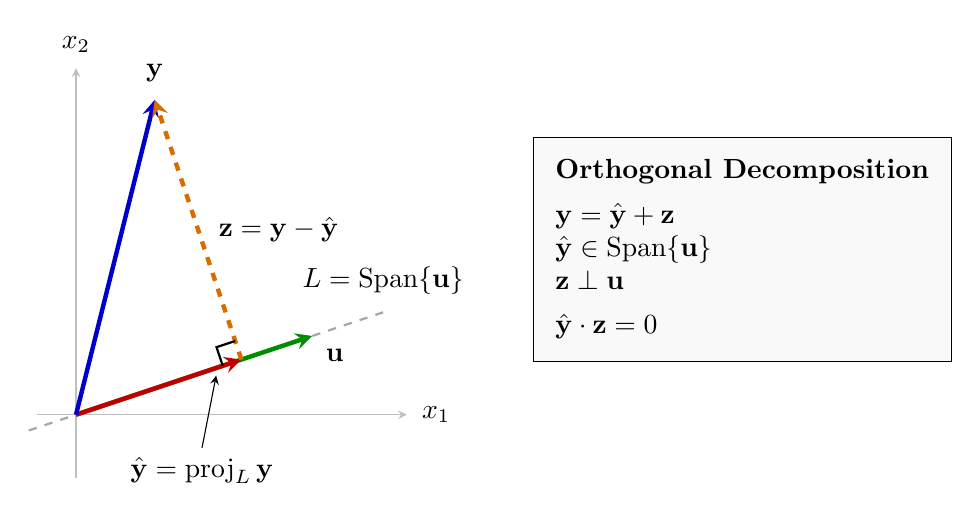
\begin{tikzpicture}[scale=1.0]
% 1. Axes and subspace line
\draw[thin, gray!50, ->, >=stealth] (-0.5, 0) -- (4.2, 0) node[right=2pt, black] {$x_1$};
\draw[thin, gray!50, ->, >=stealth] (0, -0.8) -- (0, 4.4) node[above=2pt, black] {$x_2$};
\draw[thick, gray!70, dashed] (-0.6, -0.2) -- (3.9, 1.3);

% 2. Primary vectors and right-angle marker
\draw[ultra thick, green!55!black, ->, >=stealth] (0, 0) -- (3, 1);
\draw[ultra thick, red!75!black, ->, >=stealth] (0, 0) -- (2.1, 0.7);
\draw[ultra thick, blue!80!black, ->, >=stealth] (0, 0) -- (1, 4);
\draw[ultra thick, orange!85!black, dashed, ->, >=stealth] (2.1, 0.7) -- (1, 4);
\draw[thick, black] (1.863, 0.621) -- (1.784, 0.858) -- (2.021, 0.937);

% 3. Labels, off-axis callout, and anchored legend
\node[above=3pt, black] at (1, 4) {$\mathbf{y}$};
\node[right=4pt, black] at (1.55, 2.35) {$\mathbf{z} = \mathbf{y} - \hat{\mathbf{y}}$};
\node[above=3pt, black] at (3.9, 1.3) {$L = \operatorname{Span}\{\mathbf{u}\}$};
\node[below right=2pt, black] at (3, 1) {$\mathbf{u}$};
\node[below=2pt, black] (yhatlbl) at (1.6, -0.35) {$\hat{\mathbf{y}} = \operatorname{proj}_L \mathbf{y}$};
\draw[->, >=stealth, thin, black, shorten >=3pt] (yhatlbl.north) -- (1.8, 0.6);

\node[draw=black, fill=gray!5, align=left, inner sep=8pt, anchor=west, text=black] at (5.8, 2.1) {
    \textbf{Orthogonal Decomposition}\\[4pt]
    $\mathbf{y} = \hat{\mathbf{y}} + \mathbf{z}$\\
    $\hat{\mathbf{y}} \in \operatorname{Span}\{\mathbf{u}\}$\\
    $\mathbf{z} \perp \mathbf{u}$\\[4pt]
    $\hat{\mathbf{y}} \cdot \mathbf{z} = 0$
};
\end{tikzpicture}
\end{center}

\textbf{Answer:} $\mathbf{y} = \begin{bmatrix} 21/10 \\ 7/10 \end{bmatrix} + \begin{bmatrix} -11/10 \\ 33/10 \end{bmatrix}$.

\textbf{Problem 12.} Let $W = \operatorname{Span}\{\mathbf{u}_1, \mathbf{u}_2\} \subset \mathbb{R}^3$, where $\mathbf{u}_1 = \begin{bmatrix} 1 \\ 2 \\ 0 \end{bmatrix}$ and $\mathbf{u}_2 = \begin{bmatrix} -2 \\ 1 \\ 5 \end{bmatrix}$, and let $\mathbf{y} = \begin{bmatrix} 3 \\ 1 \\ -2 \end{bmatrix}$. \\
(a) Verify that $\{\mathbf{u}_1, \mathbf{u}_2\}$ is an orthogonal basis for $W$. \\
(b) Compute $\hat{\mathbf{y}} = \operatorname{proj}_W \mathbf{y} = \frac{\mathbf{y} \cdot \mathbf{u}_1}{\mathbf{u}_1 \cdot \mathbf{u}_1}\mathbf{u}_1 + \frac{\mathbf{y} \cdot \mathbf{u}_2}{\mathbf{u}_2 \cdot \mathbf{u}_2}\mathbf{u}_2$. \\
(c) Write $\mathbf{y} = \hat{\mathbf{y}} + \mathbf{z}$, and verify explicitly that $\mathbf{z}$ is orthogonal to both $\mathbf{u}_1$ and $\mathbf{u}_2$ (hence $\mathbf{z} \in W^\perp$).

\textbf{Solution:} \\
(a) $\mathbf{u}_1 \cdot \mathbf{u}_2 = 1(-2) + 2(1) + 0(5) = 0$. Since $\mathbf{u}_1$ and $\mathbf{u}_2$ are nonzero and orthogonal, they are linearly independent and span $W$, forming an orthogonal basis for $W$. \\
(b) Compute the projection weights:
\[
\frac{\mathbf{y} \cdot \mathbf{u}_1}{\mathbf{u}_1 \cdot \mathbf{u}_1} = \frac{3(1) + 1(2) + (-2)(0)}{1^2 + 2^2 + 0^2} = \frac{5}{5} = 1, \qquad
\frac{\mathbf{y} \cdot \mathbf{u}_2}{\mathbf{u}_2 \cdot \mathbf{u}_2} = \frac{3(-2) + 1(1) + (-2)(5)}{(-2)^2 + 1^2 + 5^2} = \frac{-15}{30} = -\frac{1}{2}.
\]
Thus,
\[
\hat{\mathbf{y}} = 1\begin{bmatrix} 1 \\ 2 \\ 0 \end{bmatrix} - \frac{1}{2}\begin{bmatrix} -2 \\ 1 \\ 5 \end{bmatrix} = \begin{bmatrix} 2 \\ 3/2 \\ -5/2 \end{bmatrix}.
\]
(c) Set $\mathbf{z} = \mathbf{y} - \hat{\mathbf{y}} = \begin{bmatrix} 3 - 2 \\ 1 - 3/2 \\ -2 - (-5/2) \end{bmatrix} = \begin{bmatrix} 1 \\ -1/2 \\ 1/2 \end{bmatrix}$. Check orthogonality:
\[
\mathbf{z} \cdot \mathbf{u}_1 = 1(1) + \left(-\frac{1}{2}\right)(2) + \frac{1}{2}(0) = 0, \qquad
\mathbf{z} \cdot \mathbf{u}_2 = 1(-2) + \left(-\frac{1}{2}\right)(1) + \frac{1}{2}(5) = -2 - \frac{1}{2} + \frac{5}{2} = 0.
\]
\textbf{Answer:} $\mathbf{y} = \begin{bmatrix} 2 \\ 3/2 \\ -5/2 \end{bmatrix} + \begin{bmatrix} 1 \\ -1/2 \\ 1/2 \end{bmatrix}$.

\textbf{Problem 13.} Compute the distance from $\mathbf{y} = \begin{bmatrix} -2 \\ 9 \end{bmatrix}$ to the line $L$ through $\mathbf{u} = \begin{bmatrix} 3 \\ 4 \end{bmatrix}$ and the origin.

\textbf{Solution:} First find the orthogonal projection $\hat{\mathbf{y}}$ onto $L$:
\[
\hat{\mathbf{y}} = \frac{\mathbf{y} \cdot \mathbf{u}}{\mathbf{u} \cdot \mathbf{u}}\mathbf{u} = \frac{(-2)(3) + 9(4)}{3^2 + 4^2}\begin{bmatrix} 3 \\ 4 \end{bmatrix} = \frac{30}{25}\begin{bmatrix} 3 \\ 4 \end{bmatrix} = \frac{6}{5}\begin{bmatrix} 3 \\ 4 \end{bmatrix} = \begin{bmatrix} 18/5 \\ 24/5 \end{bmatrix}.
\]
The orthogonal error vector is $\mathbf{z} = \mathbf{y} - \hat{\mathbf{y}} = \begin{bmatrix} -10/5 - 18/5 \\ 45/5 - 24/5 \end{bmatrix} = \begin{bmatrix} -28/5 \\ 21/5 \end{bmatrix} = \frac{7}{5}\begin{bmatrix} -4 \\ 3 \end{bmatrix}$. Check: $\mathbf{z} \cdot \mathbf{u} = \frac{7}{5}(-12 + 12) = 0$. The distance from $\mathbf{y}$ to $L$ is
\[
d = \|\mathbf{z}\| = \frac{7}{5}\sqrt{(-4)^2 + 3^2} = \frac{7}{5}(5) = 7.
\]
\textbf{Answer:} $d = 7$.

\textbf{Problem 14.} Compute the distance $d$ from $\mathbf{y} = \begin{bmatrix} 3 \\ -1 \\ 5 \end{bmatrix}$ to the line $L$ through $\mathbf{u} = \begin{bmatrix} 2 \\ 1 \\ 2 \end{bmatrix}$ and the origin. Verify that the Pythagorean identity $\|\mathbf{y}\|^2 = \|\hat{\mathbf{y}}\|^2 + d^2$ holds.

\textbf{Solution:} Project $\mathbf{y}$ onto $L$:
\[
\hat{\mathbf{y}} = \frac{3(2) + (-1)(1) + 5(2)}{2^2 + 1^2 + 2^2}\begin{bmatrix} 2 \\ 1 \\ 2 \end{bmatrix} = \frac{15}{9}\begin{bmatrix} 2 \\ 1 \\ 2 \end{bmatrix} = \frac{5}{3}\begin{bmatrix} 2 \\ 1 \\ 2 \end{bmatrix} = \begin{bmatrix} 10/3 \\ 5/3 \\ 10/3 \end{bmatrix}.
\]
Then $\mathbf{z} = \mathbf{y} - \hat{\mathbf{y}} = \begin{bmatrix} 9/3 - 10/3 \\ -3/3 - 5/3 \\ 15/3 - 10/3 \end{bmatrix} = \begin{bmatrix} -1/3 \\ -8/3 \\ 5/3 \end{bmatrix}$. Check: $\mathbf{z} \cdot \mathbf{u} = \frac{-2 - 8 + 10}{3} = 0$. Thus,
\[
d = \|\mathbf{z}\| = \sqrt{\left(-\frac{1}{3}\right)^2 + \left(-\frac{8}{3}\right)^2 + \left(\frac{5}{3}\right)^2} = \sqrt{\frac{1 + 64 + 25}{9}} = \sqrt{\frac{90}{9}} = \sqrt{10}.
\]
Pythagorean verification: $\|\mathbf{y}\|^2 = 3^2 + (-1)^2 + 5^2 = 35$, $\|\hat{\mathbf{y}}\|^2 = \frac{100 + 25 + 100}{9} = \frac{225}{9} = 25$, and $d^2 = 10$, so $\|\hat{\mathbf{y}}\|^2 + d^2 = 25 + 10 = 35 = \|\mathbf{y}\|^2$. \\
\textbf{Answer:} $d = \sqrt{10}$.

\textbf{Problem 15.} Let $L = \operatorname{Span}\{\mathbf{u}\}$ in $\mathbb{R}^2$, where $\mathbf{u} = \begin{bmatrix} 2 \\ 1 \end{bmatrix}$, and let $\mathbf{y} = \begin{bmatrix} 1 \\ 3 \end{bmatrix}$. \\
(a) Compute the orthogonal reflection $\operatorname{refl}_L \mathbf{y} = 2\operatorname{proj}_L \mathbf{y} - \mathbf{y}$. \\
(b) Verify that $\|\operatorname{refl}_L \mathbf{y}\| = \|\mathbf{y}\|$ and that $\operatorname{refl}_L \mathbf{y} - \hat{\mathbf{y}} = -(\mathbf{y} - \hat{\mathbf{y}})$.

\textbf{Solution:} \\
(a) First compute $\hat{\mathbf{y}} = \operatorname{proj}_L \mathbf{y} = \frac{1(2) + 3(1)}{2^2 + 1^2}\begin{bmatrix} 2 \\ 1 \end{bmatrix} = \frac{5}{5}\begin{bmatrix} 2 \\ 1 \end{bmatrix} = \begin{bmatrix} 2 \\ 1 \end{bmatrix}$. Then
\[
\operatorname{refl}_L \mathbf{y} = 2\hat{\mathbf{y}} - \mathbf{y} = 2\begin{bmatrix} 2 \\ 1 \end{bmatrix} - \begin{bmatrix} 1 \\ 3 \end{bmatrix} = \begin{bmatrix} 3 \\ -1 \end{bmatrix}.
\]
(b) $\|\operatorname{refl}_L \mathbf{y}\| = \sqrt{3^2 + (-1)^2} = \sqrt{10}$ and $\|\mathbf{y}\| = \sqrt{1^2 + 3^2} = \sqrt{10}$, so length is preserved. Moreover, $\operatorname{refl}_L \mathbf{y} - \hat{\mathbf{y}} = \begin{bmatrix} 3 - 2 \\ -1 - 1 \end{bmatrix} = \begin{bmatrix} 1 \\ -2 \end{bmatrix} = -\begin{bmatrix} -1 \\ 2 \end{bmatrix} = -(\mathbf{y} - \hat{\mathbf{y}})$.

\begin{center}
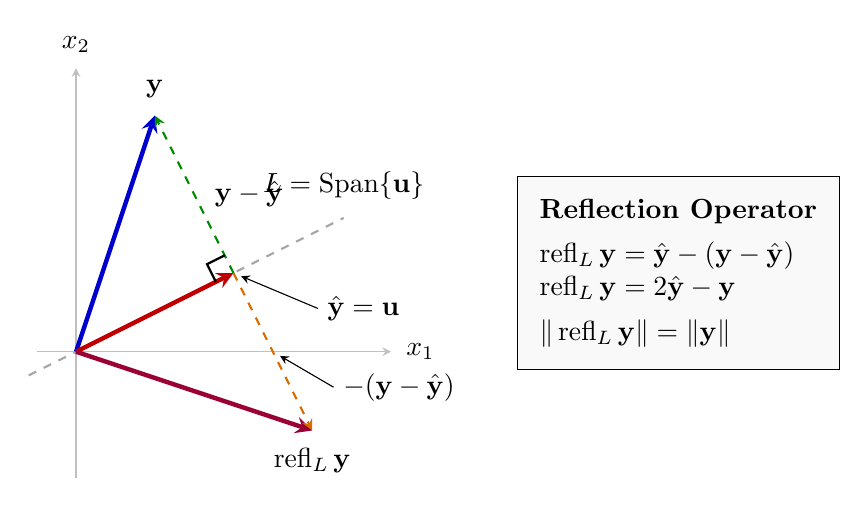
\begin{tikzpicture}[scale=1.0]
% 1. Axes and line L
\draw[thin, gray!50, ->, >=stealth] (-0.5, 0) -- (4.0, 0) node[right=2pt, black] {$x_1$};
\draw[thin, gray!50, ->, >=stealth] (0, -1.6) -- (0, 3.6) node[above=2pt, black] {$x_2$};
\draw[thick, gray!70, dashed] (-0.6, -0.3) -- (3.4, 1.7);

% 2. Primary vectors and dashed difference vectors
\draw[ultra thick, blue!80!black, ->, >=stealth] (0, 0) -- (1, 3);
\draw[ultra thick, red!75!black, ->, >=stealth] (0, 0) -- (2, 1);
\draw[ultra thick, purple!80!black, ->, >=stealth] (0, 0) -- (3, -1);
\draw[thick, green!55!black, dashed, ->, >=stealth] (2, 1) -- (1, 3);
\draw[thick, orange!85!black, dashed, ->, >=stealth] (2, 1) -- (3, -1);
\draw[thick, black] (1.776, 0.888) -- (1.664, 1.112) -- (1.888, 1.224);

% 3. Labels, callouts, and anchored legend
\node[above=3pt, black] at (1, 3) {$\mathbf{y}$};
\node[below=3pt, black] at (3, -1) {$\operatorname{refl}_L \mathbf{y}$};
\node[above=3pt, black] at (3.4, 1.7) {$L = \operatorname{Span}\{\mathbf{u}\}$};
\node[right=4pt, black] at (1.5, 2.0) {$\mathbf{y} - \hat{\mathbf{y}}$};

\node[right=2pt, black] (yhat15) at (3.0, 0.55) {$\hat{\mathbf{y}} = \mathbf{u}$};
\draw[->, >=stealth, thin, black, shorten >=3pt] (yhat15.west) -- (2, 1);

\node[right=2pt, black] (refldiff) at (3.2, -0.45) {$-(\mathbf{y} - \hat{\mathbf{y}})$};
\draw[->, >=stealth, thin, black, shorten >=3pt] (refldiff.west) -- (2.5, 0.0);

\node[draw=black, fill=gray!5, align=left, inner sep=8pt, anchor=west, text=black] at (5.6, 1.0) {
    \textbf{Reflection Operator}\\[4pt]
    $\operatorname{refl}_L \mathbf{y} = \hat{\mathbf{y}} - (\mathbf{y} - \hat{\mathbf{y}})$\\
    $\operatorname{refl}_L \mathbf{y} = 2\hat{\mathbf{y}} - \mathbf{y}$\\[4pt]
    $\|\operatorname{refl}_L \mathbf{y}\| = \|\mathbf{y}\|$
};
\end{tikzpicture}
\end{center}

\textbf{Answer:} $\operatorname{refl}_L \mathbf{y} = \begin{bmatrix} 3 \\ -1 \end{bmatrix}$.

\subsection{Solutions to Problems 16--18: Orthonormal Sets and Normalization}

\textbf{Problem 16.} Determine whether the set $\{\mathbf{v}_1, \mathbf{v}_2\}$ in $\mathbb{R}^3$ is orthonormal. If it is only orthogonal, normalize the vectors to form an orthonormal set:
\[
\mathbf{v}_1 = \begin{bmatrix} 1/2 \\ -1/2 \\ 1/2 \end{bmatrix}, \qquad
\mathbf{v}_2 = \begin{bmatrix} 1/3 \\ 1/3 \\ 0 \end{bmatrix}.
\]
\textbf{Solution:} First test orthogonality: $\mathbf{v}_1 \cdot \mathbf{v}_2 = \frac{1}{6} - \frac{1}{6} + 0 = 0$, so the set is orthogonal. Next compute the norms:
\[
\|\mathbf{v}_1\| = \sqrt{\frac{1}{4} + \frac{1}{4} + \frac{1}{4}} = \frac{\sqrt{3}}{2} \neq 1, \qquad
\|\mathbf{v}_2\| = \sqrt{\frac{1}{9} + \frac{1}{9} + 0} = \frac{\sqrt{2}}{3} \neq 1.
\]
Hence the set is orthogonal, not orthonormal. Normalizing each vector yields:
\[
\mathbf{u}_1 = \frac{\mathbf{v}_1}{\|\mathbf{v}_1\|} = \frac{2}{\sqrt{3}}\begin{bmatrix} 1/2 \\ -1/2 \\ 1/2 \end{bmatrix} = \begin{bmatrix} 1/\sqrt{3} \\ -1/\sqrt{3} \\ 1/\sqrt{3} \end{bmatrix}, \qquad
\mathbf{u}_2 = \frac{\mathbf{v}_2}{\|\mathbf{v}_2\|} = \frac{3}{\sqrt{2}}\begin{bmatrix} 1/3 \\ 1/3 \\ 0 \end{bmatrix} = \begin{bmatrix} 1/\sqrt{2} \\ 1/\sqrt{2} \\ 0 \end{bmatrix}.
\]
\textbf{Answer:} Orthogonal but not orthonormal. Normalized: $\mathbf{u}_1 = \begin{bmatrix} 1/\sqrt{3} \\ -1/\sqrt{3} \\ 1/\sqrt{3} \end{bmatrix}$, $\mathbf{u}_2 = \begin{bmatrix} 1/\sqrt{2} \\ 1/\sqrt{2} \\ 0 \end{bmatrix}$.

\textbf{Problem 17.} Determine whether the set $\{\mathbf{v}_1, \mathbf{v}_2, \mathbf{v}_3\}$ in $\mathbb{R}^3$ is orthonormal:
\[
\mathbf{v}_1 = \begin{bmatrix} 2/\sqrt{14} \\ 1/\sqrt{14} \\ -3/\sqrt{14} \end{bmatrix}, \qquad
\mathbf{v}_2 = \begin{bmatrix} 1/\sqrt{5} \\ -2/\sqrt{5} \\ 0 \end{bmatrix}, \qquad
\mathbf{v}_3 = \begin{bmatrix} 6/\sqrt{70} \\ 3/\sqrt{70} \\ 5/\sqrt{70} \end{bmatrix}.
\]
\textbf{Solution:} Check pairwise orthogonality:
\[
\mathbf{v}_1 \cdot \mathbf{v}_2 = \frac{2 - 2 + 0}{\sqrt{70}} = 0, \qquad
\mathbf{v}_1 \cdot \mathbf{v}_3 = \frac{12 + 3 - 15}{\sqrt{980}} = 0, \qquad
\mathbf{v}_2 \cdot \mathbf{v}_3 = \frac{6 - 6 + 0}{\sqrt{350}} = 0.
\]
Check squared norms:
\[
\|\mathbf{v}_1\|^2 = \frac{4 + 1 + 9}{14} = 1, \qquad
\|\mathbf{v}_2\|^2 = \frac{1 + 4 + 0}{5} = 1, \qquad
\|\mathbf{v}_3\|^2 = \frac{36 + 9 + 25}{70} = 1.
\]
All pairs are orthogonal and all vectors have unit norm. \\
\textbf{Answer:} Orthonormal.

\textbf{Problem 18.} Let $\mathbf{v}_1 = \begin{bmatrix} 1 \\ 2 \\ 2 \end{bmatrix}$ and $\mathbf{v}_2 = \begin{bmatrix} 2 \\ -1 \\ 0 \end{bmatrix}$. \\
(a) Verify that $\mathbf{v}_1$ and $\mathbf{v}_2$ are orthogonal, and normalize them to obtain unit vectors $\mathbf{u}_1$ and $\mathbf{u}_2$. \\
(b) Find a third unit vector $\mathbf{u}_3 \in \mathbb{R}^3$ with positive first entry such that $\{\mathbf{u}_1, \mathbf{u}_2, \mathbf{u}_3\}$ forms an orthonormal basis for $\mathbb{R}^3$.

\textbf{Solution:} \\
(a) $\mathbf{v}_1 \cdot \mathbf{v}_2 = 2 - 2 + 0 = 0$. Their norms are $\|\mathbf{v}_1\| = \sqrt{1 + 4 + 4} = 3$ and $\|\mathbf{v}_2\| = \sqrt{4 + 1 + 0} = \sqrt{5}$, so
\[
\mathbf{u}_1 = \begin{bmatrix} 1/3 \\ 2/3 \\ 2/3 \end{bmatrix}, \qquad
\mathbf{u}_2 = \begin{bmatrix} 2/\sqrt{5} \\ -1/\sqrt{5} \\ 0 \end{bmatrix}.
\]
(b) Seek $\mathbf{w} = \begin{bmatrix} a \\ b \\ c \end{bmatrix}$ orthogonal to $\mathbf{v}_1$ and $\mathbf{v}_2$ with $a > 0$:
\[
2a - b = 0 \implies b = 2a, \qquad
a + 2b + 2c = a + 4a + 2c = 0 \implies c = -\frac{5}{2}a.
\]
Choosing $a = 2$ gives $\mathbf{w} = \begin{bmatrix} 2 \\ 4 \\ -5 \end{bmatrix}$, with $\|\mathbf{w}\| = \sqrt{4 + 16 + 25} = \sqrt{45} = 3\sqrt{5}$. Normalizing gives
\[
\mathbf{u}_3 = \frac{\mathbf{w}}{\|\mathbf{w}\|} = \begin{bmatrix} 2/(3\sqrt{5}) \\ 4/(3\sqrt{5}) \\ -5/(3\sqrt{5}) \end{bmatrix}.
\]
\textbf{Answer:} $\mathbf{u}_1 = \begin{bmatrix} 1/3 \\ 2/3 \\ 2/3 \end{bmatrix}$, $\mathbf{u}_2 = \begin{bmatrix} 2/\sqrt{5} \\ -1/\sqrt{5} \\ 0 \end{bmatrix}$, $\mathbf{u}_3 = \begin{bmatrix} 2/(3\sqrt{5}) \\ 4/(3\sqrt{5}) \\ -5/(3\sqrt{5}) \end{bmatrix}$.

\subsection{Solutions to Problems 19--22: Conceptual Analysis (True or False)}

\textbf{Problem 19.} Determine whether each statement is True or False, and justify your answer with a proof or counterexample: \\
(a) Every linearly independent set of vectors in $\mathbb{R}^n$ is orthogonal. \\
(b) Every orthogonal set of vectors in $\mathbb{R}^n$ is linearly independent.

\textbf{Solution:} \\
(a) \textbf{False.} Counterexample: $\left\{\begin{bmatrix} 1 \\ 0 \end{bmatrix}, \begin{bmatrix} 1 \\ 1 \end{bmatrix}\right\}$ is linearly independent in $\mathbb{R}^2$, yet $\begin{bmatrix} 1 \\ 0 \end{bmatrix} \cdot \begin{bmatrix} 1 \\ 1 \end{bmatrix} = 1 \neq 0$. \\
(b) \textbf{False.} Counterexample: $\left\{\begin{bmatrix} 1 \\ 0 \end{bmatrix}, \begin{bmatrix} 0 \\ 0 \end{bmatrix}\right\}$ is orthogonal because $\mathbf{0} \cdot \mathbf{v} = 0$, yet any set containing the zero vector is linearly dependent. (Theorem 4 requires the orthogonal vectors to be \textit{nonzero}.)

\textbf{Problem 20.} Determine whether each statement is True or False, and justify your answer: \\
(a) If $\{\mathbf{v}_1, \mathbf{v}_2\}$ is an orthogonal set of nonzero vectors, then normalizing each vector preserves orthogonality and yields an orthonormal set. \\
(b) If $\{\mathbf{u}_1, \dots, \mathbf{u}_p\}$ is an orthogonal basis for a subspace $W \subseteq \mathbb{R}^n$ and $\mathbf{x} \in W$, then $\mathbf{x} = c_1\mathbf{u}_1 + \dots + c_p\mathbf{u}_p$ where $c_j = \frac{\mathbf{x} \cdot \mathbf{u}_j}{\mathbf{u}_j \cdot \mathbf{u}_j}$.

\textbf{Solution:} \\
(a) \textbf{True.} Let $\mathbf{u}_i = \mathbf{v}_i / \|\mathbf{v}_i\|$. Each $\mathbf{u}_i$ has unit length, and $\mathbf{u}_1 \cdot \mathbf{u}_2 = \frac{1}{\|\mathbf{v}_1\|\|\mathbf{v}_2\|}(\mathbf{v}_1 \cdot \mathbf{v}_2) = 0$. \\
(b) \textbf{True.} By Theorem 5, taking the dot product of $\mathbf{x} = \sum_{i=1}^p c_i \mathbf{u}_i$ with $\mathbf{u}_j$ cancels every term $i \neq j$ since $\mathbf{u}_i \cdot \mathbf{u}_j = 0$, leaving $\mathbf{x} \cdot \mathbf{u}_j = c_j(\mathbf{u}_j \cdot \mathbf{u}_j)$. Because basis vectors are nonzero, $\mathbf{u}_j \cdot \mathbf{u}_j > 0$, yielding $c_j = \frac{\mathbf{x} \cdot \mathbf{u}_j}{\mathbf{u}_j \cdot \mathbf{u}_j}$.

\textbf{Problem 21.} Determine whether each statement is True or False, and justify your answer: \\
(a) If $U$ is a $4 \times 3$ matrix with orthonormal columns, then $U$ is an orthogonal matrix and satisfies $U U^T = I_4$. \\
(b) If $U$ is an $n \times n$ matrix with orthonormal columns, then $U$ is invertible and $U^{-1} = U^T$.

\textbf{Solution:} \\
(a) \textbf{False.} By definition, an orthogonal matrix must be \textit{square}. Moreover, for a $4 \times 3$ matrix $U$ with orthonormal columns, $U^T U = I_3$, whereas $U U^T$ is a $4 \times 4$ projection matrix onto $\operatorname{Col}(U)$ of rank $3$, which cannot equal $I_4$ (rank $4$). \\
(b) \textbf{True.} Orthonormal columns give $U^T U = I_n$. Because $U$ is square, the Invertible Matrix Theorem guarantees that a square matrix with a left inverse $U^T$ is invertible and $U^{-1} = U^T$.

\textbf{Problem 22.} Determine whether each statement is True or False, and justify your answer: \\
(a) For any nonzero vector $\mathbf{v} \in \mathbb{R}^n$, any nonzero scalar $c \in \mathbb{R}$, and any $\mathbf{y} \in \mathbb{R}^n$, we have $\operatorname{proj}_{c\mathbf{v}} \mathbf{y} = \operatorname{proj}_{\mathbf{v}} \mathbf{y}$. \\
(b) For any vector $\mathbf{y} \in \mathbb{R}^n$ and any line $L = \operatorname{Span}\{\mathbf{u}\}$ with $\mathbf{u} \neq \mathbf{0}$, the distance from $\mathbf{y}$ to $L$ is $\|\operatorname{proj}_L \mathbf{y}\|$.

\textbf{Solution:} \\
(a) \textbf{True.} Direct substitution pulls out the scalar $c$:
\[
\operatorname{proj}_{c\mathbf{v}} \mathbf{y} = \frac{\mathbf{y} \cdot (c\mathbf{v})}{(c\mathbf{v}) \cdot (c\mathbf{v})}(c\mathbf{v}) = \frac{c(\mathbf{y} \cdot \mathbf{v})}{c^2(\mathbf{v} \cdot \mathbf{v})}(c\mathbf{v}) = \frac{\mathbf{y} \cdot \mathbf{v}}{\mathbf{v} \cdot \mathbf{v}}\mathbf{v} = \operatorname{proj}_{\mathbf{v}} \mathbf{y}.
\]
(b) \textbf{False.} $\|\operatorname{proj}_L \mathbf{y}\| = \|\hat{\mathbf{y}}\|$ is the distance from the origin to $\hat{\mathbf{y}}$. The distance from $\mathbf{y}$ to $L$ is $\|\mathbf{y} - \hat{\mathbf{y}}\|$.

\subsection{Solutions to Problems 23--28: Proofs, Linear Transformations, and Matrix Properties}

\textbf{Problem 23.} (a) Prove Theorem 4: If $S = \{\mathbf{v}_1, \mathbf{v}_2, \dots, \mathbf{v}_p\}$ is an orthogonal set of nonzero vectors in $\mathbb{R}^n$, then $S$ is linearly independent. \\
(b) Explain why any subspace $W \subseteq \mathbb{R}^n$ spanned by $n$ nonzero orthogonal vectors must satisfy $W = \mathbb{R}^n$.

\textbf{Solution:}
\begin{proof}
(a) Suppose $c_1\mathbf{v}_1 + c_2\mathbf{v}_2 + \dots + c_p\mathbf{v}_p = \mathbf{0}$ for scalars $c_1, \dots, c_p \in \mathbb{R}$. Fix any index $j \in \{1, \dots, p\}$ and take the dot product of both sides with $\mathbf{v}_j$:
\[
0 = \mathbf{0} \cdot \mathbf{v}_j = \left(\sum_{i=1}^p c_i \mathbf{v}_i\right) \cdot \mathbf{v}_j = \sum_{i=1}^p c_i (\mathbf{v}_i \cdot \mathbf{v}_j) = c_j(\mathbf{v}_j \cdot \mathbf{v}_j),
\]
since $\mathbf{v}_i \cdot \mathbf{v}_j = 0$ for all $i \neq j$. Because $\mathbf{v}_j \neq \mathbf{0}$, we have $\mathbf{v}_j \cdot \mathbf{v}_j = \|\mathbf{v}_j\|^2 > 0$, forcing $c_j = 0$. Since $j$ was arbitrary, $c_1 = \dots = c_p = 0$, proving linear independence.

(b) By part (a), the $n$ nonzero orthogonal vectors are linearly independent in $\mathbb{R}^n$. Because $\operatorname{dim}(\mathbb{R}^n) = n$, any linearly independent set of $n$ vectors in $\mathbb{R}^n$ forms a basis for $\mathbb{R}^n$, and therefore its span $W$ equals $\mathbb{R}^n$.
\end{proof}

\textbf{Problem 24.} Let $U$ be an $m \times n$ matrix with orthonormal columns. Using the matrix-transpose identity $\mathbf{u} \cdot \mathbf{v} = \mathbf{u}^T \mathbf{v}$, prove Theorem 7: for all $\mathbf{x}, \mathbf{y} \in \mathbb{R}^n$, \\
(a) $(U\mathbf{x}) \cdot (U\mathbf{y}) = \mathbf{x} \cdot \mathbf{y}$ (and deduce that $U\mathbf{x} \perp U\mathbf{y}$ whenever $\mathbf{x} \perp \mathbf{y}$); \\
(b) $\|U\mathbf{x}\| = \|\mathbf{x}\|$.

\textbf{Solution:}
\begin{proof}
Since $U$ has orthonormal columns, $U^T U = I_n$. \\
(a) Using $(U\mathbf{x})^T = \mathbf{x}^T U^T$, we compute
\[
(U\mathbf{x}) \cdot (U\mathbf{y}) = (U\mathbf{x})^T(U\mathbf{y}) = \mathbf{x}^T (U^T U) \mathbf{y} = \mathbf{x}^T I_n \mathbf{y} = \mathbf{x}^T \mathbf{y} = \mathbf{x} \cdot \mathbf{y}.
\]
In particular, if $\mathbf{x} \perp \mathbf{y}$, then $\mathbf{x} \cdot \mathbf{y} = 0$, so $(U\mathbf{x}) \cdot (U\mathbf{y}) = 0$, meaning $U\mathbf{x} \perp U\mathbf{y}$. \\
(b) Setting $\mathbf{y} = \mathbf{x}$ in part (a) gives $\|U\mathbf{x}\|^2 = (U\mathbf{x}) \cdot (U\mathbf{x}) = \mathbf{x} \cdot \mathbf{x} = \|\mathbf{x}\|^2$. Since norms are nonnegative, taking square roots yields $\|U\mathbf{x}\| = \|\mathbf{x}\|$.
\end{proof}

\textbf{Problem 25.} Let $U$ and $V$ be $n \times n$ orthogonal matrices (square matrices with orthonormal columns). \\
(a) Explain why $U$ is invertible and $U^{-1} = U^T$. \\
(b) Prove that the rows of $U$ form an orthonormal basis of $\mathbb{R}^n$. \\
(c) Prove that the matrix product $UV$ is also an orthogonal matrix.

\textbf{Solution:}
\begin{proof}
(a) Because $U$ has orthonormal columns, $U^T U = I_n$. Since $U$ is square ($n \times n$), the Invertible Matrix Theorem implies that a square matrix with left inverse $U^T$ is invertible with two-sided inverse $U^{-1} = U^T$.

(b) From $U^{-1} = U^T$, we also obtain $U U^T = I_n$. Rewriting this as $(U^T)^T (U^T) = I_n$ shows that $U^T$ has orthonormal columns. Since the columns of $U^T$ are the rows of $U$, the $n$ rows of $U$ form an orthonormal set in $\mathbb{R}^n$; being $n$ nonzero orthogonal vectors in $\mathbb{R}^n$, they form an orthonormal basis of $\mathbb{R}^n$.

(c) First, $UV$ is $n \times n$. Using $U^T U = I_n$ and $V^T V = I_n$:
\[
(UV)^T (UV) = (V^T U^T)(UV) = V^T (U^T U) V = V^T I_n V = V^T V = I_n.
\]
Hence $UV$ is a square matrix with orthonormal columns, so $UV$ is an orthogonal matrix.
\end{proof}

\textbf{Problem 26.} Let $\mathbf{u} \in \mathbb{R}^n$ be a nonzero vector and $L = \operatorname{Span}\{\mathbf{u}\}$. \\
(a) Prove that both $T(\mathbf{x}) = \operatorname{proj}_L \mathbf{x} = \frac{\mathbf{x} \cdot \mathbf{u}}{\mathbf{u} \cdot \mathbf{u}}\mathbf{u}$ and $R(\mathbf{x}) = 2\operatorname{proj}_L \mathbf{x} - \mathbf{x}$ are linear transformations from $\mathbb{R}^n$ to $\mathbb{R}^n$. \\
(b) Let $n = 2$ and $\mathbf{u} = \begin{bmatrix} 3 \\ 4 \end{bmatrix}$. Find the $2 \times 2$ standard matrices $[T]$ and $[R]$ such that $T(\mathbf{x}) = [T]\mathbf{x}$ and $R(\mathbf{x}) = [R]\mathbf{x}$, and verify directly that $[R]$ is an orthogonal matrix.

\textbf{Solution:} \\
(a) For any $\mathbf{x}, \mathbf{y} \in \mathbb{R}^n$ and $c \in \mathbb{R}$, linearity of the dot product gives:
\begin{align*}
T(\mathbf{x} + \mathbf{y}) &= \frac{(\mathbf{x} + \mathbf{y}) \cdot \mathbf{u}}{\mathbf{u} \cdot \mathbf{u}}\mathbf{u} = \frac{\mathbf{x} \cdot \mathbf{u}}{\mathbf{u} \cdot \mathbf{u}}\mathbf{u} + \frac{\mathbf{y} \cdot \mathbf{u}}{\mathbf{u} \cdot \mathbf{u}}\mathbf{u} = T(\mathbf{x}) + T(\mathbf{y}), \\
T(c\mathbf{x}) &= \frac{(c\mathbf{x}) \cdot \mathbf{u}}{\mathbf{u} \cdot \mathbf{u}}\mathbf{u} = c\frac{\mathbf{x} \cdot \mathbf{u}}{\mathbf{u} \cdot \mathbf{u}}\mathbf{u} = cT(\mathbf{x}).
\end{align*}
Thus $T$ is linear. Since $R(\mathbf{x}) = 2T(\mathbf{x}) - I(\mathbf{x})$ is a linear combination of the linear transformations $T$ and the identity $I$, $R$ is also linear. \\
(b) Here $\mathbf{u} \cdot \mathbf{u} = 3^2 + 4^2 = 25$. Computing images of the standard basis vectors $\mathbf{e}_1, \mathbf{e}_2$:
\[
T(\mathbf{e}_1) = \frac{3}{25}\begin{bmatrix} 3 \\ 4 \end{bmatrix} = \begin{bmatrix} 9/25 \\ 12/25 \end{bmatrix}, \qquad
T(\mathbf{e}_2) = \frac{4}{25}\begin{bmatrix} 3 \\ 4 \end{bmatrix} = \begin{bmatrix} 12/25 \\ 16/25 \end{bmatrix},
\]
so $[T] = \frac{1}{25}\begin{bmatrix} 9 & 12 \\ 12 & 16 \end{bmatrix}$. Then $[R] = 2[T] - I_2 = \frac{1}{25}\begin{bmatrix} 18 - 25 & 24 \\ 24 & 32 - 25 \end{bmatrix} = \frac{1}{25}\begin{bmatrix} -7 & 24 \\ 24 & 7 \end{bmatrix}$. Verification:
\[
[R]^T [R] = \frac{1}{625}\begin{bmatrix} -7 & 24 \\ 24 & 7 \end{bmatrix}\begin{bmatrix} -7 & 24 \\ 24 & 7 \end{bmatrix} = \frac{1}{625}\begin{bmatrix} 49 + 576 & -168 + 168 \\ -168 + 168 & 576 + 49 \end{bmatrix} = \begin{bmatrix} 1 & 0 \\ 0 & 1 \end{bmatrix} = I_2,
\]
confirming that $[R]$ is an orthogonal matrix. \\
\textbf{Answer:} $[T] = \frac{1}{25}\begin{bmatrix} 9 & 12 \\ 12 & 16 \end{bmatrix}$, $[R] = \frac{1}{25}\begin{bmatrix} -7 & 24 \\ 24 & 7 \end{bmatrix}$.

\textbf{Problem 27.} Let $A = \begin{bmatrix} 1 & -2 \\ 2 & -1 \\ 2 & 2 \end{bmatrix}$. Observe that the columns of $A$ are orthogonal, and let $U$ be the $3 \times 2$ matrix obtained by normalizing each column of $A$. \\
(a) Compute $U$, $U^T U$, and $U U^T$. Explain why $U^T U = I_2$ while $U U^T \neq I_3$. \\
(b) For an arbitrary vector $\mathbf{y} \in \mathbb{R}^3$, let $\mathbf{p} = U U^T \mathbf{y}$ and $\mathbf{z} = \mathbf{y} - \mathbf{p}$. Prove in general that $\mathbf{p} \in \operatorname{Col}(A)$ and $\mathbf{z} \in (\operatorname{Col}(A))^\perp$. \\
(c) Compute $\mathbf{p}$ and $\mathbf{z}$ explicitly for $\mathbf{y} = \begin{bmatrix} 3 \\ 3 \\ 9 \end{bmatrix}$ and verify that $\mathbf{z}$ is orthogonal to both columns of $A$.

\textbf{Solution:} \\
(a) Each column of $A$ has norm $\sqrt{1 + 4 + 4} = 3$ and $\sqrt{4 + 1 + 4} = 3$, with $\mathbf{a}_1 \cdot \mathbf{a}_2 = -2 - 2 + 4 = 0$. Normalizing gives
\[
U = \frac{1}{3}\begin{bmatrix} 1 & -2 \\ 2 & -1 \\ 2 & 2 \end{bmatrix}, \qquad
U^T U = \frac{1}{9}\begin{bmatrix} 1 & 2 & 2 \\ -2 & -1 & 2 \end{bmatrix}\begin{bmatrix} 1 & -2 \\ 2 & -1 \\ 2 & 2 \end{bmatrix} = \frac{1}{9}\begin{bmatrix} 9 & 0 \\ 0 & 9 \end{bmatrix} = I_2,
\]
\[
U U^T = \frac{1}{9}\begin{bmatrix} 1 & -2 \\ 2 & -1 \\ 2 & 2 \end{bmatrix}\begin{bmatrix} 1 & 2 & 2 \\ -2 & -1 & 2 \end{bmatrix} = \frac{1}{9}\begin{bmatrix} 5 & 4 & -2 \\ 4 & 5 & 2 \\ -2 & 2 & 8 \end{bmatrix}.
\]
Here $U^T U = I_2$ because the two columns of $U$ are orthonormal. However, $U$ is $3 \times 2$ (not square), so $U U^T$ is the rank-$2$ projection matrix onto $\operatorname{Col}(A)$ and cannot equal $I_3$ (rank $3$). \\
(b) Since $\mathbf{p} = U(U^T \mathbf{y})$, $\mathbf{p}$ is a linear combination of the columns of $U$. Because each column of $U$ is a nonzero scalar multiple of the corresponding column of $A$, $\operatorname{Col}(U) = \operatorname{Col}(A)$, so $\mathbf{p} \in \operatorname{Col}(A)$. Next,
\[
U^T \mathbf{z} = U^T(\mathbf{y} - U U^T \mathbf{y}) = U^T \mathbf{y} - (U^T U)U^T \mathbf{y} = U^T \mathbf{y} - I_2 U^T \mathbf{y} = \mathbf{0}.
\]
Hence $\mathbf{z}$ is orthogonal to every column of $U$, and therefore orthogonal to every vector in $\operatorname{Col}(A)$, proving $\mathbf{z} \in (\operatorname{Col}(A))^\perp$. \\
(c) For $\mathbf{y} = \begin{bmatrix} 3 \\ 3 \\ 9 \end{bmatrix}$,
\[
\mathbf{p} = U U^T \mathbf{y} = \frac{1}{9}\begin{bmatrix} 5 & 4 & -2 \\ 4 & 5 & 2 \\ -2 & 2 & 8 \end{bmatrix}\begin{bmatrix} 3 \\ 3 \\ 9 \end{bmatrix} = \frac{1}{9}\begin{bmatrix} 15 + 12 - 18 \\ 12 + 15 + 18 \\ -6 + 6 + 72 \end{bmatrix} = \begin{bmatrix} 1 \\ 5 \\ 8 \end{bmatrix}, \qquad
\mathbf{z} = \mathbf{y} - \mathbf{p} = \begin{bmatrix} 2 \\ -2 \\ 1 \end{bmatrix}.
\]
Check: $\mathbf{z} \cdot \mathbf{a}_1 = 2 - 4 + 2 = 0$ and $\mathbf{z} \cdot \mathbf{a}_2 = -4 + 2 + 2 = 0$. \\
\textbf{Answer:} $\mathbf{p} = \begin{bmatrix} 1 \\ 5 \\ 8 \end{bmatrix}$, $\mathbf{z} = \begin{bmatrix} 2 \\ -2 \\ 1 \end{bmatrix}$.

\textbf{Problem 28.} Let $A$ be any $m \times n$ matrix with columns $\mathbf{a}_1, \mathbf{a}_2, \dots, \mathbf{a}_n \in \mathbb{R}^m$. \\
(a) Prove that the $(i, j)$-entry of $A^T A$ equals $\mathbf{a}_i \cdot \mathbf{a}_j$. \\
(b) Deduce that the columns of $A$ form an orthogonal set if and only if $A^T A$ is a diagonal matrix. \\
(c) Deduce that the columns of $A$ form an orthonormal set if and only if $A^T A = I_n$.

\textbf{Solution:}
\begin{proof}
(a) The $i$-th row of $A^T$ is $\mathbf{a}_i^T$ and the $j$-th column of $A$ is $\mathbf{a}_j$. By definition of matrix multiplication,
\[
(A^T A)_{ij} = (\text{row } i \text{ of } A^T)(\text{col } j \text{ of } A) = \mathbf{a}_i^T \mathbf{a}_j = \mathbf{a}_i \cdot \mathbf{a}_j.
\]
(b) The columns of $A$ are mutually orthogonal if and only if $\mathbf{a}_i \cdot \mathbf{a}_j = 0$ for all $i \neq j$. By part (a), this holds if and only if $(A^T A)_{ij} = 0$ for all $i \neq j$, which is the exact definition of $A^T A$ being a diagonal matrix.

(c) The columns of $A$ form an orthonormal set if and only if $\mathbf{a}_i \cdot \mathbf{a}_j = 0$ for all $i \neq j$ and $\mathbf{a}_i \cdot \mathbf{a}_i = \|\mathbf{a}_i\|^2 = 1$ for all $i$. By part (a), this occurs if and only if $A^T A = I_n$.
\end{proof}

\subsection{Solutions to Problems 29--33: Advanced Applications}

\textbf{Problem 29.} Let $W = \operatorname{Span}\{\mathbf{x}_1, \mathbf{x}_2\} \subset \mathbb{R}^3$, where $\mathbf{x}_1 = \begin{bmatrix} 1 \\ 2 \\ 2 \end{bmatrix}$ and $\mathbf{x}_2 = \begin{bmatrix} 3 \\ 0 \\ 3 \end{bmatrix}$. Use the Gram-Schmidt process to find: \\
(a) an orthogonal basis $\{\mathbf{v}_1, \mathbf{v}_2\}$ for $W$; \\
(b) an orthonormal basis $\{\mathbf{u}_1, \mathbf{u}_2\}$ for $W$.

\textbf{Solution:} \\
(a) Set $\mathbf{v}_1 = \mathbf{x}_1 = \begin{bmatrix} 1 \\ 2 \\ 2 \end{bmatrix}$, so $\mathbf{v}_1 \cdot \mathbf{v}_1 = 1 + 4 + 4 = 9$. Then
\[
\mathbf{v}_2 = \mathbf{x}_2 - \frac{\mathbf{x}_2 \cdot \mathbf{v}_1}{\mathbf{v}_1 \cdot \mathbf{v}_1}\mathbf{v}_1 = \begin{bmatrix} 3 \\ 0 \\ 3 \end{bmatrix} - \frac{3 + 0 + 6}{9}\begin{bmatrix} 1 \\ 2 \\ 2 \end{bmatrix} = \begin{bmatrix} 3 \\ 0 \\ 3 \end{bmatrix} - \begin{bmatrix} 1 \\ 2 \\ 2 \end{bmatrix} = \begin{bmatrix} 2 \\ -2 \\ 1 \end{bmatrix}.
\]
Check: $\mathbf{v}_1 \cdot \mathbf{v}_2 = 2 - 4 + 2 = 0$. \\
(b) Since $\|\mathbf{v}_1\| = 3$ and $\|\mathbf{v}_2\| = \sqrt{4 + 4 + 1} = 3$, normalizing yields
\[
\mathbf{u}_1 = \begin{bmatrix} 1/3 \\ 2/3 \\ 2/3 \end{bmatrix}, \qquad
\mathbf{u}_2 = \begin{bmatrix} 2/3 \\ -2/3 \\ 1/3 \end{bmatrix}.
\]
\textbf{Answer:} (a) $\left\{\begin{bmatrix} 1 \\ 2 \\ 2 \end{bmatrix}, \begin{bmatrix} 2 \\ -2 \\ 1 \end{bmatrix}\right\}$. (b) $\left\{\begin{bmatrix} 1/3 \\ 2/3 \\ 2/3 \end{bmatrix}, \begin{bmatrix} 2/3 \\ -2/3 \\ 1/3 \end{bmatrix}\right\}$.

\textbf{Problem 30.} Apply the Gram-Schmidt process to the linearly independent set $\{\mathbf{x}_1, \mathbf{x}_2, \mathbf{x}_3\}$ in $\mathbb{R}^3$ to construct an orthogonal basis $\{\mathbf{v}_1, \mathbf{v}_2, \mathbf{v}_3\}$ for $\mathbb{R}^3$, where
\[
\mathbf{x}_1 = \begin{bmatrix} 1 \\ 1 \\ 0 \end{bmatrix}, \qquad
\mathbf{x}_2 = \begin{bmatrix} 2 \\ 0 \\ 1 \end{bmatrix}, \qquad
\mathbf{x}_3 = \begin{bmatrix} 1 \\ 3 \\ 5 \end{bmatrix}.
\]
Verify directly that all pairwise dot products among $\mathbf{v}_1, \mathbf{v}_2, \mathbf{v}_3$ equal zero.

\textbf{Solution:} \\
Step 1: $\mathbf{v}_1 = \mathbf{x}_1 = \begin{bmatrix} 1 \\ 1 \\ 0 \end{bmatrix}$, with $\mathbf{v}_1 \cdot \mathbf{v}_1 = 2$. \\
Step 2: $\mathbf{v}_2 = \mathbf{x}_2 - \frac{\mathbf{x}_2 \cdot \mathbf{v}_1}{\mathbf{v}_1 \cdot \mathbf{v}_1}\mathbf{v}_1 = \begin{bmatrix} 2 \\ 0 \\ 1 \end{bmatrix} - \frac{2}{2}\begin{bmatrix} 1 \\ 1 \\ 0 \end{bmatrix} = \begin{bmatrix} 1 \\ -1 \\ 1 \end{bmatrix}$, with $\mathbf{v}_2 \cdot \mathbf{v}_2 = 3$. \\
Step 3: Compute $\mathbf{x}_3 \cdot \mathbf{v}_1 = 1 + 3 + 0 = 4$ and $\mathbf{x}_3 \cdot \mathbf{v}_2 = 1 - 3 + 5 = 3$. Subtract both projections:
\[
\mathbf{v}_3 = \mathbf{x}_3 - \frac{\mathbf{x}_3 \cdot \mathbf{v}_1}{\mathbf{v}_1 \cdot \mathbf{v}_1}\mathbf{v}_1 - \frac{\mathbf{x}_3 \cdot \mathbf{v}_2}{\mathbf{v}_2 \cdot \mathbf{v}_2}\mathbf{v}_2 = \begin{bmatrix} 1 \\ 3 \\ 5 \end{bmatrix} - \frac{4}{2}\begin{bmatrix} 1 \\ 1 \\ 0 \end{bmatrix} - \frac{3}{3}\begin{bmatrix} 1 \\ -1 \\ 1 \end{bmatrix} = \begin{bmatrix} -2 \\ 2 \\ 4 \end{bmatrix}.
\]
Verification: $\mathbf{v}_1 \cdot \mathbf{v}_2 = 1 - 1 + 0 = 0$, $\mathbf{v}_1 \cdot \mathbf{v}_3 = -2 + 2 + 0 = 0$, and $\mathbf{v}_2 \cdot \mathbf{v}_3 = -2 - 2 + 4 = 0$. \\
\textbf{Answer:} $\mathbf{v}_1 = \begin{bmatrix} 1 \\ 1 \\ 0 \end{bmatrix}$, $\mathbf{v}_2 = \begin{bmatrix} 1 \\ -1 \\ 1 \end{bmatrix}$, $\mathbf{v}_3 = \begin{bmatrix} -2 \\ 2 \\ 4 \end{bmatrix}$.

\textbf{Problem 31.} Let $A = \begin{bmatrix} 1 & 0 \\ 1 & 1 \\ 0 & 1 \end{bmatrix}$, whose columns are linearly independent but not orthogonal. \\
(a) Compute the standard projection matrix $P = A(A^T A)^{-1}A^T$ onto $\operatorname{Col}(A)$. \\
(b) Verify directly that $P^2 = P$ and $P^T = P$, and use $P$ to compute the projection $\hat{\mathbf{y}} = P\mathbf{y}$ of $\mathbf{y} = \begin{bmatrix} 3 \\ 0 \\ 3 \end{bmatrix}$ onto $\operatorname{Col}(A)$. \\
(c) Prove algebraically that if $U$ is any $m \times n$ matrix with orthonormal columns, then $P_U = U U^T$ satisfies $P_U^2 = P_U$ and $P_U^T = P_U$, and explain why $A(A^T A)^{-1} A^T$ collapses to $U U^T$ when $A = U$.

\textbf{Solution:} \\
(a) Compute $A^T A$ and its inverse:
\[
A^T A = \begin{bmatrix} 1 & 1 & 0 \\ 0 & 1 & 1 \end{bmatrix}\begin{bmatrix} 1 & 0 \\ 1 & 1 \\ 0 & 1 \end{bmatrix} = \begin{bmatrix} 2 & 1 \\ 1 & 2 \end{bmatrix}, \qquad
(A^T A)^{-1} = \frac{1}{3}\begin{bmatrix} 2 & -1 \\ -1 & 2 \end{bmatrix}.
\]
Multiply sequentially:
\[
A(A^T A)^{-1} = \frac{1}{3}\begin{bmatrix} 1 & 0 \\ 1 & 1 \\ 0 & 1 \end{bmatrix}\begin{bmatrix} 2 & -1 \\ -1 & 2 \end{bmatrix} = \frac{1}{3}\begin{bmatrix} 2 & -1 \\ 1 & 1 \\ -1 & 2 \end{bmatrix}, \qquad
P = \frac{1}{3}\begin{bmatrix} 2 & -1 \\ 1 & 1 \\ -1 & 2 \end{bmatrix}\begin{bmatrix} 1 & 1 & 0 \\ 0 & 1 & 1 \end{bmatrix} = \frac{1}{3}\begin{bmatrix} 2 & 1 & -1 \\ 1 & 2 & 1 \\ -1 & 1 & 2 \end{bmatrix}.
\]
(b) By inspection, $P^T = P$. Squaring gives
\[
P^2 = \frac{1}{9}\begin{bmatrix} 2 & 1 & -1 \\ 1 & 2 & 1 \\ -1 & 1 & 2 \end{bmatrix}\begin{bmatrix} 2 & 1 & -1 \\ 1 & 2 & 1 \\ -1 & 1 & 2 \end{bmatrix} = \frac{1}{9}\begin{bmatrix} 6 & 3 & -3 \\ 3 & 6 & 3 \\ -3 & 3 & 6 \end{bmatrix} = \frac{1}{3}\begin{bmatrix} 2 & 1 & -1 \\ 1 & 2 & 1 \\ -1 & 1 & 2 \end{bmatrix} = P.
\]
For $\mathbf{y} = \begin{bmatrix} 3 \\ 0 \\ 3 \end{bmatrix}$, $\hat{\mathbf{y}} = P\mathbf{y} = \frac{1}{3}\begin{bmatrix} 6 - 3 \\ 3 + 3 \\ -3 + 6 \end{bmatrix} = \begin{bmatrix} 1 \\ 2 \\ 1 \end{bmatrix}$. (Check: $\mathbf{y} - \hat{\mathbf{y}} = \begin{bmatrix} 2 \\ -2 \\ 2 \end{bmatrix}$ is orthogonal to both columns of $A$.) \\
(c) Using $U^T U = I_n$:
\[
P_U^T = (U U^T)^T = (U^T)^T U^T = U U^T = P_U, \qquad
P_U^2 = (U U^T)(U U^T) = U(U^T U)U^T = U I_n U^T = U U^T = P_U.
\]
When $A = U$, $A^T A = U^T U = I_n$, so $(A^T A)^{-1} = I_n$ and $A(A^T A)^{-1}A^T = U I_n U^T = U U^T$. \\
\textbf{Answer:} $P = \frac{1}{3}\begin{bmatrix} 2 & 1 & -1 \\ 1 & 2 & 1 \\ -1 & 1 & 2 \end{bmatrix}$, $\hat{\mathbf{y}} = \begin{bmatrix} 1 \\ 2 \\ 1 \end{bmatrix}$.

\textbf{Problem 32.} In an Ordinary Least Squares (OLS) regression problem with $N = 4$ observations and $p = 2$ features, the design matrix $X \in \mathbb{R}^{4 \times 2}$ and target vector $\mathbf{y} \in \mathbb{R}^4$ are
\[
X = \begin{bmatrix} 1 & 0 \\ 1 & 1 \\ 1 & 2 \\ 1 & 3 \end{bmatrix}, \qquad
\mathbf{y} = \begin{bmatrix} 2 \\ 2 \\ 4 \\ 8 \end{bmatrix}.
\]
We seek a parameter vector $\hat{\boldsymbol{\beta}} \in \mathbb{R}^2$ minimizing the squared error loss $\mathcal{L}(\boldsymbol{\beta}) = \|\mathbf{y} - X\boldsymbol{\beta}\|^2$. \\
(a) Using the geometric condition that the residual $\boldsymbol{\epsilon} = \mathbf{y} - X\hat{\boldsymbol{\beta}}$ must be orthogonal to $\operatorname{Col}(X)$, derive the Normal Equations $X^T X \hat{\boldsymbol{\beta}} = X^T \mathbf{y}$. \\
(b) Solve the Normal Equations to find $\hat{\boldsymbol{\beta}}$. \\
(c) Compute the fitted vector $\hat{\mathbf{y}} = X\hat{\boldsymbol{\beta}}$ and residual vector $\boldsymbol{\epsilon} = \mathbf{y} - \hat{\mathbf{y}}$, and verify explicitly that $X^T \boldsymbol{\epsilon} = \mathbf{0}$. \\
(d) Explain how the Normal Equations simplify if a feature matrix $Q \in \mathbb{R}^{4 \times 2}$ has orthonormal columns instead.

\textbf{Solution:} \\
(a) Minimizing $\|\mathbf{y} - X\boldsymbol{\beta}\|^2$ places $X\hat{\boldsymbol{\beta}}$ as the orthogonal projection of $\mathbf{y}$ onto $\operatorname{Col}(X)$, meaning $\boldsymbol{\epsilon} = \mathbf{y} - X\hat{\boldsymbol{\beta}}$ is orthogonal to every column of $X$. Equivalently,
\[
X^T \boldsymbol{\epsilon} = \mathbf{0} \implies X^T(\mathbf{y} - X\hat{\boldsymbol{\beta}}) = \mathbf{0} \implies X^T X \hat{\boldsymbol{\beta}} = X^T \mathbf{y}.
\]
(b) Compute $X^T X$ and $X^T \mathbf{y}$:
\[
X^T X = \begin{bmatrix} 1 & 1 & 1 & 1 \\ 0 & 1 & 2 & 3 \end{bmatrix}\begin{bmatrix} 1 & 0 \\ 1 & 1 \\ 1 & 2 \\ 1 & 3 \end{bmatrix} = \begin{bmatrix} 4 & 6 \\ 6 & 14 \end{bmatrix}, \qquad
X^T \mathbf{y} = \begin{bmatrix} 1 & 1 & 1 & 1 \\ 0 & 1 & 2 & 3 \end{bmatrix}\begin{bmatrix} 2 \\ 2 \\ 4 \\ 8 \end{bmatrix} = \begin{bmatrix} 16 \\ 34 \end{bmatrix}.
\]
Since $\det(X^T X) = 56 - 36 = 20$,
\[
\hat{\boldsymbol{\beta}} = (X^T X)^{-1} X^T \mathbf{y} = \frac{1}{20}\begin{bmatrix} 14 & -6 \\ -6 & 4 \end{bmatrix}\begin{bmatrix} 16 \\ 34 \end{bmatrix} = \frac{1}{20}\begin{bmatrix} 224 - 204 \\ -96 + 136 \end{bmatrix} = \begin{bmatrix} 1 \\ 2 \end{bmatrix}.
\]
(c) The fitted vector is $\hat{\mathbf{y}} = X\hat{\boldsymbol{\beta}} = \begin{bmatrix} 1 \\ 3 \\ 5 \\ 7 \end{bmatrix}$, and the residual is $\boldsymbol{\epsilon} = \mathbf{y} - \hat{\mathbf{y}} = \begin{bmatrix} 1 \\ -1 \\ -1 \\ 1 \end{bmatrix}$. Check:
\[
X^T \boldsymbol{\epsilon} = \begin{bmatrix} 1 & 1 & 1 & 1 \\ 0 & 1 & 2 & 3 \end{bmatrix}\begin{bmatrix} 1 \\ -1 \\ -1 \\ 1 \end{bmatrix} = \begin{bmatrix} 1 - 1 - 1 + 1 \\ 0 - 1 - 2 + 3 \end{bmatrix} = \begin{bmatrix} 0 \\ 0 \end{bmatrix} = \mathbf{0}.
\]
(d) If $Q$ has orthonormal columns, $Q^T Q = I_2$, so the Normal Equations $Q^T Q \hat{\boldsymbol{\beta}} = Q^T \mathbf{y}$ collapse to $\hat{\boldsymbol{\beta}} = Q^T \mathbf{y}$, completely decoupling the parameter estimates just as in Theorem 5. \\
\textbf{Answer:} $\hat{\boldsymbol{\beta}} = \begin{bmatrix} 1 \\ 2 \end{bmatrix}$, $\hat{\mathbf{y}} = \begin{bmatrix} 1 \\ 3 \\ 5 \\ 7 \end{bmatrix}$, $\boldsymbol{\epsilon} = \begin{bmatrix} 1 \\ -1 \\ -1 \\ 1 \end{bmatrix}$.

\textbf{Problem 33.} In calculus, the inner product of two continuous functions $f$ and $g$ on $[-\pi, \pi]$ is defined by
\[
\langle f, g \rangle = \int_{-\pi}^{\pi} f(x)g(x)\,dx.
\]
(a) Verify that $\{1, \cos(x), \sin(x)\}$ is an orthogonal set under this inner product by computing $\langle 1, \cos(x) \rangle$, $\langle 1, \sin(x) \rangle$, and $\langle \cos(x), \sin(x) \rangle$. \\
(b) Compute the squared norms $\langle 1, 1 \rangle$, $\langle \cos(x), \cos(x) \rangle$, and $\langle \sin(x), \sin(x) \rangle$. \\
(c) Using the decoupled orthogonal projection weights $c_j = \frac{\langle h, u_j \rangle}{\langle u_j, u_j \rangle}$, compute the orthogonal projection $\hat{h}(x)$ of $h(x) = 3 + x$ onto $\operatorname{Span}\{1, \cos(x), \sin(x)\}$.

\textbf{Solution:} \\
(a) Evaluating the integrals on $[-\pi, \pi]$:
\begin{align*}
\langle 1, \cos(x) \rangle &= \int_{-\pi}^{\pi} \cos(x)\,dx = \bigl[\sin(x)\bigr]_{-\pi}^{\pi} = 0, \\
\langle 1, \sin(x) \rangle &= \int_{-\pi}^{\pi} \sin(x)\,dx = \bigl[-\cos(x)\bigr]_{-\pi}^{\pi} = 0, \\
\langle \cos(x), \sin(x) \rangle &= \frac{1}{2}\int_{-\pi}^{\pi} \sin(2x)\,dx = \left[-\frac{1}{4}\cos(2x)\right]_{-\pi}^{\pi} = 0.
\end{align*}
(b) Compute the squared norms:
\begin{align*}
\langle 1, 1 \rangle &= \int_{-\pi}^{\pi} 1\,dx = 2\pi, \\
\langle \cos(x), \cos(x) \rangle &= \int_{-\pi}^{\pi} \frac{1 + \cos(2x)}{2}\,dx = \left[\frac{x}{2} + \frac{\sin(2x)}{4}\right]_{-\pi}^{\pi} = \pi, \\
\langle \sin(x), \sin(x) \rangle &= \int_{-\pi}^{\pi} \frac{1 - \cos(2x)}{2}\,dx = \left[\frac{x}{2} - \frac{\sin(2x)}{4}\right]_{-\pi}^{\pi} = \pi.
\end{align*}
(c) Compute the three projection coefficients independently for $h(x) = 3 + x$:
\begin{align*}
c_1 &= \frac{\langle 3 + x, 1 \rangle}{2\pi} = \frac{1}{2\pi}\int_{-\pi}^{\pi} (3 + x)\,dx = \frac{6\pi + 0}{2\pi} = 3, \\
c_2 &= \frac{\langle 3 + x, \cos(x) \rangle}{\pi} = \frac{1}{\pi}\left(3\int_{-\pi}^{\pi}\cos(x)\,dx + \int_{-\pi}^{\pi} x\cos(x)\,dx\right) = 0 \quad \text{(since $x\cos(x)$ is odd)}, \\
c_3 &= \frac{\langle 3 + x, \sin(x) \rangle}{\pi} = \frac{1}{\pi}\int_{-\pi}^{\pi} x\sin(x)\,dx = \frac{1}{\pi}\left(\bigl[-x\cos(x)\bigr]_{-\pi}^{\pi} + \int_{-\pi}^{\pi}\cos(x)\,dx\right) = \frac{\pi - (-\pi)}{\pi} = 2.
\end{align*}
\textbf{Answer:} $\hat{h}(x) = 3 + 2\sin(x)$.

\subsection{Solutions to Problems 34--36: Diagnostic Testing (``Find the Flaw'')}

\textbf{Problem 34.} A student is asked to find the orthogonal projection $\hat{\mathbf{y}}$ of $\mathbf{y} = \begin{bmatrix} 4 \\ 3 \end{bmatrix}$ onto the line $L = \operatorname{Span}\{\mathbf{u}\}$ with $\mathbf{u} = \begin{bmatrix} 1 \\ 2 \end{bmatrix}$, and then compute the distance from $\mathbf{y}$ to $L$. Examine the student's work below, identify \textit{all} errors, explain why each step is mathematically invalid, and provide the corrected solution.
\begin{quote}
\textit{Student's Work:}
\[
\hat{\mathbf{y}} = \frac{\mathbf{y} \cdot \mathbf{u}}{\mathbf{y} \cdot \mathbf{y}}\mathbf{u} = \frac{4 + 6}{16 + 9}\begin{bmatrix} 1 \\ 2 \end{bmatrix} = \frac{10}{25}\begin{bmatrix} 1 \\ 2 \end{bmatrix} = \begin{bmatrix} 2/5 \\ 4/5 \end{bmatrix}.
\]
Therefore, the distance from $\mathbf{y}$ to $L$ is $\|\hat{\mathbf{y}}\| = \sqrt{(2/5)^2 + (4/5)^2} = \frac{2\sqrt{5}}{5}$.
\end{quote}
\textbf{Solution:} \\
\textbf{Error 1 (Wrong Denominator):} The projection formula onto $\mathbf{u}$ is $\hat{\mathbf{y}} = \frac{\mathbf{y} \cdot \mathbf{u}}{\mathbf{u} \cdot \mathbf{u}}\mathbf{u}$, not $\frac{\mathbf{y} \cdot \mathbf{u}}{\mathbf{y} \cdot \mathbf{y}}\mathbf{u}$. Dividing by $\mathbf{u} \cdot \mathbf{u}$ is required so that $(\mathbf{y} - \hat{\mathbf{y}}) \cdot \mathbf{u} = 0$ and the projection is invariant under scaling $\mathbf{u}$. \\
\textbf{Error 2 (Wrong Distance Vector):} The distance from $\mathbf{y}$ to $L$ is the length of the orthogonal error component, $\|\mathbf{y} - \hat{\mathbf{y}}\|$, whereas $\|\hat{\mathbf{y}}\|$ measures the distance from the origin to $\hat{\mathbf{y}}$. \\
\textbf{Corrected Solution:}
\[
\hat{\mathbf{y}} = \frac{\mathbf{y} \cdot \mathbf{u}}{\mathbf{u} \cdot \mathbf{u}}\mathbf{u} = \frac{4(1) + 3(2)}{1^2 + 2^2}\begin{bmatrix} 1 \\ 2 \end{bmatrix} = \frac{10}{5}\begin{bmatrix} 1 \\ 2 \end{bmatrix} = \begin{bmatrix} 2 \\ 4 \end{bmatrix}.
\]
The orthogonal component is $\mathbf{z} = \mathbf{y} - \hat{\mathbf{y}} = \begin{bmatrix} 4 - 2 \\ 3 - 4 \end{bmatrix} = \begin{bmatrix} 2 \\ -1 \end{bmatrix}$ (check: $\mathbf{z} \cdot \mathbf{u} = 2 - 2 = 0$), so the distance is $d = \|\mathbf{z}\| = \sqrt{2^2 + (-1)^2} = \sqrt{5}$.

\textbf{Problem 35.} A student is asked to express $\mathbf{x} = \begin{bmatrix} 8 \\ 1 \end{bmatrix}$ as a linear combination of $\mathbf{u}_1 = \begin{bmatrix} 1 \\ 2 \end{bmatrix}$ and $\mathbf{u}_2 = \begin{bmatrix} 3 \\ 1 \end{bmatrix}$. Examine the student's work below, identify the fundamental conceptual error, explain why it occurs, and provide the completely corrected solution.
\begin{quote}
\textit{Student's Work:} Using the orthogonal basis coordinate formula,
\[
c_1 = \frac{\mathbf{x} \cdot \mathbf{u}_1}{\mathbf{u}_1 \cdot \mathbf{u}_1} = \frac{8 + 2}{1 + 4} = 2, \qquad
c_2 = \frac{\mathbf{x} \cdot \mathbf{u}_2}{\mathbf{u}_2 \cdot \mathbf{u}_2} = \frac{24 + 1}{9 + 1} = \frac{5}{2}.
\]
Hence, $\mathbf{x} = 2\mathbf{u}_1 + \frac{5}{2}\mathbf{u}_2$.
\end{quote}
\textbf{Solution:} \\
\textbf{Error (Misapplying Theorem 5 to a Non-Orthogonal Basis):} The decoupled weight formula $c_i = \frac{\mathbf{x} \cdot \mathbf{u}_i}{\mathbf{u}_i \cdot \mathbf{u}_i}$ only holds when the basis is \textit{orthogonal}. Here $\mathbf{u}_1 \cdot \mathbf{u}_2 = 1(3) + 2(1) = 5 \neq 0$, so cross-terms do not vanish when taking dot products. (Indeed, $2\mathbf{u}_1 + \frac{5}{2}\mathbf{u}_2 = \begin{bmatrix} 19/2 \\ 13/2 \end{bmatrix} \neq \mathbf{x}$.) \\
\textbf{Corrected Solution:} Solve the linear system $c_1\mathbf{u}_1 + c_2\mathbf{u}_2 = \mathbf{x}$ via row reduction:
\[
\left[\begin{array}{cc|c}
1 & 3 & 8 \\
2 & 1 & 1
\end{array}\right]
\xrightarrow{R_2 \leftarrow R_2 - 2R_1}
\left[\begin{array}{cc|c}
1 & 3 & 8 \\
0 & -5 & -15
\end{array}\right]
\implies c_2 = 3, \quad c_1 = 8 - 3(3) = -1.
\]
Verification: $-1\begin{bmatrix} 1 \\ 2 \end{bmatrix} + 3\begin{bmatrix} 3 \\ 1 \end{bmatrix} = \begin{bmatrix} 8 \\ 1 \end{bmatrix} = \mathbf{x}$. Thus, $\mathbf{x} = -\mathbf{u}_1 + 3\mathbf{u}_2$.

\textbf{Problem 36.} A student is asked: (i) to determine whether $S = \left\{\begin{bmatrix} 2 \\ -1 \end{bmatrix}, \begin{bmatrix} 1 \\ 2 \end{bmatrix}\right\}$ is an orthonormal set, and (ii) to compute $M^T M$ and $N^T N$ for $M = \begin{bmatrix} 2 & 1 \\ -1 & 2 \end{bmatrix}$ and $N = \begin{bmatrix} 1 & 2 \\ 0 & 1 \end{bmatrix}$. Examine the student's work below, identify \textit{all} errors, explain why each claim fails, and provide the corrected solutions.
\begin{quote}
\textit{Student's Work:} \\
(i) Since $\begin{bmatrix} 2 \\ -1 \end{bmatrix} \cdot \begin{bmatrix} 1 \\ 2 \end{bmatrix} = 2 - 2 = 0$, the vectors are orthogonal, so $S$ is an orthonormal set. \\
(ii) Because $M$ and $N$ are both $2 \times 2$ square matrices, by the Orthogonal Matrix Property, $M^T M = I_2$ and $N^T N = I_2$.
\end{quote}
\textbf{Solution:} \\
\textbf{Error 1 (Part (i) --- Omitting Unit Length):} Orthogonality alone does not make a set orthonormal; each vector must also have unit length ($\|\mathbf{v}\| = 1$). Here $\left\|\begin{bmatrix} 2 \\ -1 \end{bmatrix}\right\| = \sqrt{5} \neq 1$ and $\left\|\begin{bmatrix} 1 \\ 2 \end{bmatrix}\right\| = \sqrt{5} \neq 1$, so $S$ is orthogonal, \textit{not} orthonormal. \\
\textbf{Error 2 (Part (ii) --- Assuming Any Square Matrix Satisfies $U^T U = I$):} The identity $U^T U = I_n$ requires $U$ to have \textit{orthonormal columns}, not merely to be square. Matrix $M$ has orthogonal columns of length $\sqrt{5} \neq 1$, while $N$ has columns that are neither orthogonal ($1\cdot 2 + 0\cdot 1 = 2 \neq 0$) nor unit length. \\
\textbf{Corrected Computations:}
\[
M^T M = \begin{bmatrix} 2 & -1 \\ 1 & 2 \end{bmatrix}\begin{bmatrix} 2 & 1 \\ -1 & 2 \end{bmatrix} = \begin{bmatrix} 5 & 0 \\ 0 & 5 \end{bmatrix} = 5I_2 \neq I_2, \qquad
N^T N = \begin{bmatrix} 1 & 0 \\ 2 & 1 \end{bmatrix}\begin{bmatrix} 1 & 2 \\ 0 & 1 \end{bmatrix} = \begin{bmatrix} 1 & 2 \\ 2 & 5 \end{bmatrix} \neq I_2.
\]

\newpage

\section{Summary Concept Checklist and Question Reference}

For rapid review and targeted practice, the full concept checklist and corresponding question numbers are reproduced below.

\renewcommand{\arraystretch}{1.5}
\begin{tabularx}{\textwidth}{>{\raggedright\arraybackslash}p{4.3cm} >{\raggedright\arraybackslash}X >{\raggedright\arraybackslash}p{2.6cm}}
\toprule
\textbf{Concept / Problem Type} & \textbf{Core Formulas, Techniques, and Pitfalls} & \textbf{Relevant Problems} \\
\midrule
Determining Orthogonal Sets \& Parameters & Check all pairwise dot products $\mathbf{v}_i \cdot \mathbf{v}_j = 0$ ($i \neq j$); solve parameter constraints and verify every pair. & 1, 2, 3, 4 \\
\addlinespace[4pt]
The Zero Vector Trap \& Linear Independence & Since $\mathbf{0} \cdot \mathbf{v} = 0$ for all $\mathbf{v}$, a set containing $\mathbf{0}$ can be orthogonal, but is never linearly independent or orthonormal. & 3, 19, 23 \\
\addlinespace[4pt]
Orthogonal Bases \& Decoupled Weights (Theorems 4 \& 5) & Nonzero orthogonal vectors are linearly independent; basis weights decouple cleanly as $c_i = \frac{\mathbf{x} \cdot \mathbf{u}_i}{\mathbf{u}_i \cdot \mathbf{u}_i}$ without row reduction. & 5, 6, 7, 8, 20, 23, 35 \\
\addlinespace[4pt]
Orthogonal Projections onto Lines \& Subspaces & Compute $\hat{\mathbf{y}} = \operatorname{proj}_L \mathbf{y} = \frac{\mathbf{y} \cdot \mathbf{u}}{\mathbf{u} \cdot \mathbf{u}}\mathbf{u}$; scaling invariance $\operatorname{proj}_{c\mathbf{u}}\mathbf{y} = \operatorname{proj}_{\mathbf{u}}\mathbf{y}$ ($c \neq 0$); multi-vector orthogonal projection. & 9, 10, 12, 22, 26, 34 \\
\addlinespace[4pt]
Orthogonal Decomposition \& Error Check & Decompose $\mathbf{y} = \hat{\mathbf{y}} + \mathbf{z}$ with $\hat{\mathbf{y}} \in W$ and $\mathbf{z} = \mathbf{y} - \hat{\mathbf{y}} \in W^\perp$; always verify $\mathbf{z} \cdot \mathbf{u}_i = 0$. & 11, 12, 27 \\
\addlinespace[4pt]
Distance to a Subspace \& Pythagorean Theorem & Distance is $d = \|\mathbf{y} - \hat{\mathbf{y}}\| = \|\mathbf{z}\|$ (never $\|\hat{\mathbf{y}}\|$); satisfies $\|\mathbf{y}\|^2 = \|\hat{\mathbf{y}}\|^2 + \|\mathbf{z}\|^2$. & 13, 14, 22, 34 \\
\addlinespace[4pt]
Reflection Operators \& Linear Transformations & $\operatorname{refl}_L \mathbf{y} = 2\operatorname{proj}_L \mathbf{y} - \mathbf{y}$; prove linearity of $\operatorname{proj}_L$ and $\operatorname{refl}_L$, compute standard matrices, and verify $\|\operatorname{refl}_L \mathbf{y}\| = \|\mathbf{y}\|$. & 15, 26 \\
\addlinespace[4pt]
Orthonormal Sets \& Normalization & Requires orthogonality \textit{and} unit length ($\|\mathbf{u}_i\| = 1$); normalize via $\mathbf{u}_i = \mathbf{v}_i / \|\mathbf{v}_i\|$, which preserves orthogonality. & 16, 17, 18, 20, 36 \\
\addlinespace[4pt]
Norm \& Inner Product Preservation (Theorem 7) & If $U$ has orthonormal columns ($U^T U = I_n$), then $(U\mathbf{x}) \cdot (U\mathbf{y}) = \mathbf{x} \cdot \mathbf{y}$ and $\|U\mathbf{x}\| = \|\mathbf{x}\|$. & 24, 28 \\
\addlinespace[4pt]
Square Orthogonal Matrices ($U^{-1} = U^T$) & Must be square ($n \times n$); $U^T U = U U^T = I_n$; invertible with $U^{-1} = U^T$; orthonormal rows; closed under multiplication ($UV$). & 21, 25, 26, 36 \\
\addlinespace[4pt]
Rectangular Matrices ($U^T U$ vs.\ $U U^T$) & For $m \times n$ ($m > n$), $U^T U = I_n$ while $U U^T \neq I_m$ projects onto $\operatorname{Col}(A)$; $(A^T A)_{ij} = \mathbf{a}_i \cdot \mathbf{a}_j$ determines orthogonality. & 21, 27, 28, 31 \\
\addlinespace[4pt]
The Gram-Schmidt Process & Convert a non-orthogonal basis to an orthogonal basis via $\mathbf{v}_k = \mathbf{x}_k - \sum_{i=1}^{k-1} \frac{\mathbf{x}_k \cdot \mathbf{v}_i}{\mathbf{v}_i \cdot \mathbf{v}_i}\mathbf{v}_i$, then normalize if needed. & 29, 30 \\
\addlinespace[4pt]
General Projection Matrices & Compute $P = A(A^T A)^{-1}A^T$, verify $P^2 = P$ and $P^T = P$, and show $P$ collapses to $U U^T$ for orthonormal columns. & 27, 31 \\
\addlinespace[4pt]
Ordinary Least Squares (OLS) \& Normal Equations & Minimize $\|\mathbf{y} - X\boldsymbol{\beta}\|^2$ via $X^T \boldsymbol{\epsilon} = \mathbf{0} \implies X^T X \hat{\boldsymbol{\beta}} = X^T \mathbf{y}$; simplifies to $\hat{\boldsymbol{\beta}} = Q^T \mathbf{y}$ when $Q$ has orthonormal columns. & 32 \\
\addlinespace[4pt]
Integral Inner Products \& Fourier Decoupling & Verify orthogonality of $\{1, \cos(x), \sin(x)\}$ under $\langle f, g \rangle = \int_{-\pi}^{\pi} f(x)g(x)\,dx$ and project functions using Theorem 5 weights. & 33 \\
\addlinespace[4pt]
Diagnostic Testing (``Find the Flaw'') & Identify wrong projection denominators ($\mathbf{y}\cdot\mathbf{y}$), wrong distance norms ($\|\hat{\mathbf{y}}\|$), Theorem 5 on non-orthogonal bases, and $U^T U = I$ traps. & 34, 35, 36 \\
\bottomrule
\end{tabularx}

\end{document}